\section{Energy Consumption Over Time}\label{app:timeseries}

This section illustrated how the energy consumption of both macrobenchmarks evolved for DUT 2, used in \cref{subsec:exp_three}. 3DM and PCM were plotted with two and all cores, illustrating the difference additional resources made. 

Measurements for 3DM were illustrated in \cref{fig:exp_3_dut_2_3dm_timeseries_all_cores} and \cref{fig:exp_3_dut_1_3dm_timeseries_two_cores} for both two and ten cores there was a startup period until $~14$ seconds, after which the benchmark started. On ten cores,  the load was on $~25$ watts for $~18$ seconds, while for two cores the energy consumption was on $12$ watts for $60$ seconds. 

\begin{figure}[H]
    \centering



\begin{tikzpicture}
    \pgfplotsset{
        width=1.0\textwidth,
        height=0.25\textheight
    }
    \begin{axis}[
        % title={Temperature dependence of CuSO\(_4\cdot\)5H\(_2\)O solubility},
        xlabel={Time (s)},
        ylabel={Energy Consumption (w)},
        xmin=0, xmax=80,
        ymin=0, ymax=30,
        % xtick={0,20,40,60,80,100},
        % ytick={0,20,40,60,80,100,120},
        legend pos=north west,
        ymajorgrids=true,
        grid style=dashed,
    ]
    
    \addplot[
        color=blue,
        % mark=square,
        ]
        coordinates {
            (0.06699943542480469, 6.203000068664551)
            (0.1830005645751953, 5.951000213623047)
            (0.29400062561035156, 7.8429999351501465)
            (0.40399932861328125, 9.815999984741211)
            (0.5, 9.371000289916992)
            (0.61199951171875, 7.958000183105469)
            (0.7210006713867188, 10.909000396728516)
            (0.8330001831054688, 7.781000137329102)
            (0.944000244140625, 8.862000465393066)
            (1.0550003051757812, 7.760000228881836)
            (1.1580009460449219, 7.763000011444092)
            (1.2770004272460938, 7.6479997634887695)
            (1.3740005493164062, 7.795000076293945)
            (1.4990005493164062, 7.7769999504089355)
            (1.5949993133544922, 7.758999824523926)
            (1.7059993743896484, 7.5920000076293945)
            (1.8180007934570312, 7.571000099182129)
            (1.9300003051757812, 7.877999782562256)
            (2.0419998168945312, 7.51800012588501)
            (2.1529998779296875, 7.60699987411499)
            (2.2649993896484375, 7.514999866485596)
            (2.3770008087158203, 7.619999885559082)
            (2.4890003204345703, 7.683000087738037)
            (2.599000930786133, 7.534999847412109)
            (2.711000442504883, 7.948999881744385)
            (2.822999954223633, 7.956999778747559)
            (2.934999465942383, 7.7769999504089355)
            (3.0470008850097656, 8.190999984741211)
            (3.1590003967285156, 12.050999641418457)
            (3.270000457763672, 15.38700008392334)
            (3.381000518798828, 11.416999816894531)
            (3.490999221801758, 13.366999626159668)
            (3.6030006408691406, 11.019000053405762)
            (3.7150001525878906, 9.763999938964844)
            (3.8269996643066406, 7.848999977111816)
            (3.920999526977539, 8.807999610900879)
            (4.033000946044922, 8.220999717712402)
            (4.143999099731445, 7.906000137329102)
            (4.256000518798828, 7.833000183105469)
            (4.368000030517578, 8.098999977111816)
            (4.479999542236328, 7.96999979019165)
            (4.591999053955078, 7.818999767303467)
            (4.701999664306641, 7.763000011444092)
            (4.798000335693359, 7.859000205993652)
            (4.909000396728516, 7.940999984741211)
            (5.020000457763672, 8.027999877929688)
            (5.131999969482422, 7.810999870300293)
            (5.243999481201172, 7.9079999923706055)
            (5.354999542236328, 8.026000022888184)
            (5.466999053955078, 7.8379998207092285)
            (5.579000473022461, 7.947999954223633)
            (5.690999984741211, 7.854000091552734)
            (5.802000045776367, 7.829999923706055)
            (5.913999557495117, 7.915999889373779)
            (6.025999069213867, 7.974999904632568)
            (6.13800048828125, 7.815999984741211)
            (6.25, 7.8460001945495605)
            (6.36199951171875, 7.919000148773193)
            (6.474000930786133, 7.848999977111816)
            (6.586000442504883, 8.020999908447266)
            (6.697999954223633, 7.8470001220703125)
            (6.809999465942383, 7.934000015258789)
            (6.920999526977539, 8.029999732971191)
            (7.033000946044922, 8.02299976348877)
            (7.143999099731445, 7.85699987411499)
            (7.256000518798828, 7.829999923706055)
            (7.368000030517578, 7.9679999351501465)
            (7.479999542236328, 7.811999797821045)
            (7.591999053955078, 7.988999843597412)
            (7.687999725341797, 7.855999946594238)
            (7.799999237060547, 7.835999965667725)
            (7.91200065612793, 7.954999923706055)
            (8.022998809814453, 7.860000133514404)
            (8.134998321533203, 7.980000019073486)
            (8.247001647949219, 7.815999984741211)
            (8.359001159667969, 7.952000141143799)
            (8.471000671386719, 7.8420000076293945)
            (8.583000183105469, 7.992000102996826)
            (8.694999694824219, 7.831999778747559)
            (8.806999206542969, 7.833000183105469)
            (8.918998718261719, 8.156000137329102)
            (9.030998229980469, 7.798999786376953)
            (9.143001556396484, 7.936999797821045)
            (9.255001068115234, 7.855000019073486)
            (9.367000579833984, 7.953000068664551)
            (9.47800064086914, 7.938000202178955)
            (9.59000015258789, 8.185999870300293)
            (9.70199966430664, 7.861000061035156)
            (9.81399917602539, 7.890999794006348)
            (9.92599868774414, 7.952000141143799)
            (10.03799819946289, 7.98799991607666)
            (10.148998260498047, 8.071000099182129)
            (10.259998321533203, 8.102999687194824)
            (10.37099838256836, 8.154000282287598)
            (10.483001708984375, 7.284999847412109)
            (10.578998565673828, 7.396999835968018)
            (10.691001892089844, 7.74399995803833)
            (10.801998138427734, 7.573999881744385)
            (10.91299819946289, 8.967000007629395)
            (11.023998260498047, 8.352999687194824)
            (11.136001586914062, 8.461000442504883)
            (11.248001098632812, 8.345999717712402)
            (11.342998504638672, 8.371999740600586)
            (11.455001831054688, 8.237000465393066)
            (11.567001342773438, 8.241000175476074)
            (11.679000854492188, 8.343000411987305)
            (11.791000366210938, 8.329000473022461)
            (11.902000427246094, 8.871999740600586)
            (12.013999938964844, 8.215999603271484)
            (12.125999450683594, 8.479999542236328)
            (12.237998962402344, 8.347000122070312)
            (12.3489990234375, 8.39900016784668)
            (12.46099853515625, 8.295999526977539)
            (12.573001861572266, 8.348999977111816)
            (12.681999206542969, 8.623000144958496)
            (12.793998718261719, 9.083999633789062)
            (12.889999389648438, 9.282999992370605)
            (13.001998901367188, 9.196000099182129)
            (13.113998413085938, 8.88599967956543)
            (13.226001739501953, 9.057999610900879)
            (13.342998504638672, 8.704000473022461)
            (13.450000762939453, 8.831000328063965)
            (13.562000274658203, 10.888999938964844)
            (13.687000274658203, 22.43199920654297)
            (13.79800033569336, 22.645999908447266)
            (13.909000396728516, 22.545000076293945)
            (14.020000457763672, 22.82200050354004)
            (14.131000518798828, 22.60099983215332)
            (14.243000030517578, 19.180999755859375)
            (14.354999542236328, 25.854999542236328)
            (14.465999603271484, 25.924999237060547)
            (14.57699966430664, 25.6200008392334)
            (14.672000885009766, 25.71500015258789)
            (14.783000946044922, 25.538999557495117)
            (14.894001007080078, 25.64900016784668)
            (15.006000518798828, 25.527000427246094)
            (15.118000030517578, 25.07200050354004)
            (15.229999542236328, 24.929000854492188)
            (15.352001190185547, 25.562000274658203)
            (15.452999114990234, 22.965999603271484)
            (15.566001892089844, 25.756999969482422)
            (15.678001403808594, 25.878000259399414)
            (15.78900146484375, 25.55900001525879)
            (15.900001525878906, 25.738000869750977)
            (16.012001037597656, 25.291000366210938)
            (16.123001098632812, 24.29800033569336)
            (16.23400115966797, 24.71299934387207)
            (16.345001220703125, 23.993000030517578)
            (16.457000732421875, 23.54400062561035)
            (16.56800079345703, 23.99799919128418)
            (16.68000030517578, 23.722000122070312)
            (16.79199981689453, 24.885000228881836)
            (16.902999877929688, 25.06999969482422)
            (17.014999389648438, 24.889999389648438)
            (17.126998901367188, 25.107999801635742)
            (17.23699951171875, 24.683000564575195)
            (17.3489990234375, 24.642000198364258)
            (17.46099853515625, 24.38800048828125)
            (17.570999145507812, 24.246000289916992)
            (17.682998657226562, 24.73699951171875)
            (17.794998168945312, 24.823999404907227)
            (17.904998779296875, 25.42799949645996)
            (18.014999389648438, 25.312000274658203)
            (18.125999450683594, 25.413000106811523)
            (18.23699951171875, 25.302000045776367)
            (18.3489990234375, 25.81100082397461)
            (18.46099853515625, 25.79199981689453)
            (18.573001861572266, 25.341999053955078)
            (18.685001373291016, 25.128999710083008)
            (18.78099822998047, 25.900999069213867)
            (18.893001556396484, 25.79599952697754)
            (19.00400161743164, 25.4689998626709)
            (19.115001678466797, 24.860000610351562)
            (19.226001739501953, 24.9689998626709)
            (19.347999572753906, 25.336999893188477)
            (19.446998596191406, 24.58099937438965)
            (19.558998107910156, 24.388999938964844)
            (19.669998168945312, 24.099000930786133)
            (19.779998779296875, 24.445999145507812)
            (19.875999450683594, 25.5)
            (19.98699951171875, 25.43000030517578)
            (20.0989990234375, 25.209999084472656)
            (20.21099853515625, 24.948999404907227)
            (20.320999145507812, 24.913000106811523)
            (20.43000030517578, 24.785999298095703)
            (20.541000366210938, 24.94700050354004)
            (20.652000427246094, 24.78700065612793)
            (20.76300048828125, 24.131999969482422)
            (20.873001098632812, 23.875999450683594)
            (20.96900177001953, 25.035999298095703)
            (21.08100128173828, 25.665000915527344)
            (21.19300079345703, 25.89299964904785)
            (21.30500030517578, 25.80500030517578)
            (21.41699981689453, 25.479999542236328)
            (21.527999877929688, 24.993000030517578)
            (21.639999389648438, 25.163999557495117)
            (21.750999450683594, 24.82699966430664)
            (21.862998962402344, 24.332000732421875)
            (21.972999572753906, 24.18899917602539)
            (22.083999633789062, 24.910999298095703)
            (22.195999145507812, 24.738000869750977)
            (22.307998657226562, 24.231000900268555)
            (22.419998168945312, 25.23699951171875)
            (22.532001495361328, 25.19499969482422)
            (22.644001007080078, 25.030000686645508)
            (22.755001068115234, 25.16699981689453)
            (22.867000579833984, 24.67300033569336)
            (22.979000091552734, 25.031999588012695)
            (23.090999603271484, 24.743000030517578)
            (23.20199966430664, 24.71299934387207)
            (23.31399917602539, 24.39900016784668)
            (23.42599868774414, 23.983999252319336)
            (23.536998748779297, 24.320999145507812)
            (23.648998260498047, 23.972000122070312)
            (23.759998321533203, 23.59600067138672)
            (23.87099838256836, 23.966999053955078)
            (23.983001708984375, 23.58099937438965)
            (24.09400177001953, 23.343000411987305)
            (24.205001831054688, 23.128000259399414)
            (24.317001342773438, 24.742000579833984)
            (24.428001403808594, 24.926000595092773)
            (24.53900146484375, 24.843000411987305)
            (24.650001525878906, 24.868000030517578)
            (24.759998321533203, 24.283000946044922)
            (24.869998931884766, 23.621000289916992)
            (24.981998443603516, 23.780000686645508)
            (25.092998504638672, 23.77899932861328)
            (25.187999725341797, 22.763999938964844)
            (25.298999786376953, 24.180999755859375)
            (25.410999298095703, 25.04400062561035)
            (25.522998809814453, 24.915000915527344)
            (25.63399887084961, 25.065000534057617)
            (25.74599838256836, 24.336999893188477)
            (25.858001708984375, 23.323999404907227)
            (25.970001220703125, 24.07900047302246)
            (26.08100128173828, 23.858999252319336)
            (26.19300079345703, 23.895999908447266)
            (26.304000854492188, 23.551000595092773)
            (26.416000366210938, 23.59000015258789)
            (26.527000427246094, 25.128000259399414)
            (26.637001037597656, 25.35099983215332)
            (26.749000549316406, 24.940000534057617)
            (26.85900115966797, 24.256999969482422)
            (26.97100067138672, 23.75200080871582)
            (27.08300018310547, 23.860000610351562)
            (27.194000244140625, 23.48900032043457)
            (27.305999755859375, 23.886999130249023)
            (27.416000366210938, 23.731000900268555)
            (27.5260009765625, 24.23900032043457)
            (27.637001037597656, 25.516000747680664)
            (27.748001098632812, 25.069000244140625)
            (27.842998504638672, 24.15399932861328)
            (27.955001831054688, 23.906999588012695)
            (28.066001892089844, 23.367000579833984)
            (28.176998138427734, 23.88800048828125)
            (28.28799819946289, 23.40399932861328)
            (28.398998260498047, 24.743000030517578)
            (28.50899887084961, 25.413999557495117)
            (28.62099838256836, 25.263999938964844)
            (28.733001708984375, 24.89699935913086)
            (28.842998504638672, 24.106000900268555)
            (28.953998565673828, 23.711999893188477)
            (29.066001892089844, 23.507999420166016)
            (29.176998138427734, 23.736000061035156)
            (29.28900146484375, 23.881999969482422)
            (29.400001525878906, 24.974000930786133)
            (29.512001037597656, 25.357999801635742)
            (29.62200164794922, 25.472000122070312)
            (29.731998443603516, 23.625)
            (29.842998504638672, 23.698999404907227)
            (29.955001831054688, 23.888999938964844)
            (30.067001342773438, 23.841999053955078)
            (30.178001403808594, 24.393999099731445)
            (30.290000915527344, 24.575000762939453)
            (30.4010009765625, 25.47800064086914)
            (30.51300048828125, 25.40999984741211)
            (30.624000549316406, 24.38800048828125)
            (30.720001220703125, 22.927000045776367)
            (30.83100128173828, 24.266000747680664)
            (30.941001892089844, 23.437000274658203)
            (31.053001403808594, 23.774999618530273)
            (31.165000915527344, 25.351999282836914)
            (31.2760009765625, 25.222999572753906)
            (31.387001037597656, 25.020000457763672)
            (31.498001098632812, 23.37299919128418)
            (31.610000610351562, 24.041000366210938)
            (31.72100067138672, 23.243000030517578)
            (31.832000732421875, 23.284000396728516)
            (31.944000244140625, 23.323999404907227)
            (32.05400085449219, 24.41699981689453)
            (32.165000915527344, 25.257999420166016)
            (32.277000427246094, 25.047000885009766)
            (32.38800048828125, 14.817999839782715)
            (32.483001708984375, 8.517000198364258)
            (32.595001220703125, 8.104000091552734)
            (32.70600128173828, 8.029999732971191)
            (32.81800079345703, 7.99399995803833)
            (32.93000030517578, 9.029999732971191)
            (33.04199981689453, 7.566999912261963)
            (33.15399932861328, 7.576000213623047)
            (33.26599884033203, 7.36899995803833)
            (33.37799835205078, 7.901000022888184)
            (33.4900016784668, 7.433000087738037)
            (33.60200119018555, 7.34499979019165)
            (33.7140007019043, 7.232999801635742)
            (33.82600021362305, 7.473999977111816)
            (33.922000885009766, 8.118000030517578)
            (34.034000396728516, 7.327000141143799)
            (34.14500045776367, 7.315999984741211)
            (34.25699996948242, 7.408999919891357)
            (34.375999450683594, 7.698999881744385)
            (34.47999954223633, 7.480000019073486)
            (34.59199905395508, 7.447999954223633)
            (34.70199966430664, 7.3520002365112305)
            (34.81399917602539, 7.236999988555908)
            (34.92599868774414, 8.46500015258789)
            (35.03799819946289, 7.296999931335449)
            (35.150001525878906, 7.27400016784668)
            (35.262001037597656, 7.302999973297119)
            (35.38199996948242, 7.625)
            (35.486000061035156, 7.302000045776367)
            (35.597999572753906, 7.263999938964844)
            (35.709999084472656, 7.329999923706055)
            (35.821998596191406, 7.433000087738037)
            (35.933998107910156, 9.005999565124512)
            (36.04600143432617, 7.710999965667725)
            (36.15800094604492, 7.61299991607666)
            (36.27000045776367, 7.330999851226807)
            (36.38999938964844, 7.611999988555908)
            (36.492000579833984, 7.452000141143799)
            (36.60300064086914, 7.370999813079834)
            (36.71500015258789, 7.438000202178955)
            (36.82699966430664, 7.454999923706055)
            (36.93899917602539, 9.314000129699707)
            (37.05099868774414, 7.348999977111816)
            (37.16299819946289, 7.276000022888184)
            (37.27399826049805, 7.372000217437744)
            (37.39400100708008, 7.783999919891357)
            (37.49700164794922, 7.5)
            (37.60900115966797, 7.269999980926514)
            (37.72100067138672, 7.401000022888184)
            (37.83300018310547, 7.593999862670898)
            (37.94499969482422, 9.597999572753906)
            (38.05699920654297, 7.557000160217285)
            (38.16899871826172, 8.449000358581543)
            (38.28099822998047, 9.258999824523926)
            (38.391998291015625, 9.680999755859375)
            (38.50199890136719, 6.0269999504089355)
            (38.61399841308594, 5.50600004196167)
            (38.72600173950195, 5.326000213623047)
            (38.8380012512207, 5.459000110626221)
            (38.95000076293945, 7.734000205993652)
            (39.0620002746582, 5.617000102996826)
            (39.17399978637695, 5.460999965667725)
            (39.2859992980957, 5.453000068664551)
            (39.39799880981445, 5.689000129699707)
            (39.5099983215332, 5.660999774932861)
            (39.62200164794922, 5.429999828338623)
            (39.731998443603516, 5.886000156402588)
            (39.84299850463867, 5.5279998779296875)
            (39.95399856567383, 6.361000061035156)
            (40.06500244140625, 6.625)
            (40.17400360107422, 6.038000106811523)
            (40.288002014160156, 6.140999794006348)
            (40.39099884033203, 6.440000057220459)
            (40.50800323486328, 6.701000213623047)
            (40.621002197265625, 7.229000091552734)
            (40.733001708984375, 5.558000087738037)
            (40.84400177001953, 8.204000473022461)
            (40.95600128173828, 9.022000312805176)
            (41.06700134277344, 10.74899959564209)
            (41.17400360107422, 11.982000350952148)
            (41.290000915527344, 9.946000099182129)
            (41.391998291015625, 10.163999557495117)
            (41.49199676513672, 10.237000465393066)
            
        };
        % \legend{CuSO\(_4\cdot\)5H\(_2\)O}
        
    \end{axis}
    \end{tikzpicture}
    \caption{A timeseries of the energy consumption over time for DUT 2 when running 3DM for all cores}
    \label{fig:exp_3_dut_2_3dm_timeseries_all_cores}
\end{figure}
\begin{figure}[H]
    \centering



\begin{tikzpicture}
    \pgfplotsset{
        width=1.0\textwidth,
        height=0.25\textheight
    }
    \begin{axis}[
        % title={Temperature dependence of CuSO\(_4\cdot\)5H\(_2\)O solubility},
        xlabel={Time (s)},
        ylabel={Energy Consumption (w)},
        xmin=0, xmax=81,
        ymin=0, ymax=30,
        % xtick={0,20,40,60,80,100},
        % ytick={0,20,40,60,80,100,120},
        legend pos=north west,
        ymajorgrids=true,
        grid style=dashed,
    ]
    
    \addplot[
        color=blue,
        % mark=square,
        ]
        coordinates {
            (0.082000732421875, 8.246000289916992)
            (0.18199920654296875, 6.13700008392334)
            (0.2950000762939453, 8.753999710083008)
            (0.39999961853027344, 6.885000228881836)
            (0.5219993591308594, 9.680000305175781)
            (0.6159992218017578, 10.79800033569336)
            (0.7280006408691406, 9.675999641418457)
            (0.8390007019042969, 9.845000267028809)
            (0.9500007629394531, 10.434000015258789)
            (1.0629997253417969, 8.38599967956543)
            (1.1749992370605469, 7.803999900817871)
            (1.2830009460449219, 7.925000190734863)
            (1.3829994201660156, 7.65500020980835)
            (1.4939994812011719, 7.895999908447266)
            (1.6060009002685547, 7.620999813079834)
            (1.7180004119873047, 7.560999870300293)
            (1.8299999237060547, 7.576000213623047)
            (1.9400005340576172, 7.833000183105469)
            (2.0510005950927734, 7.732999801635742)
            (2.1620006561279297, 7.6020002365112305)
            (2.2579994201660156, 7.679999828338623)
            (2.3700008392333984, 7.559000015258789)
            (2.4820003509521484, 7.513000011444092)
            (2.5939998626708984, 7.64900016784668)
            (2.7059993743896484, 7.47599983215332)
            (2.8180007934570312, 7.49399995803833)
            (2.9290008544921875, 8.199000358581543)
            (3.0410003662109375, 8.031000137329102)
            (3.1529998779296875, 8.012999534606934)
            (3.2649993896484375, 8.133999824523926)
            (3.3759994506835938, 10.47599983215332)
            (3.4880008697509766, 11.335000038146973)
            (3.6000003814697266, 10.657999992370605)
            (3.7119998931884766, 10.185999870300293)
            (3.8239994049072266, 10.5649995803833)
            (3.9360008239746094, 10.760000228881836)
            (4.048000335693359, 10.430000305175781)
            (4.159999847412109, 9.338000297546387)
            (4.271999359130859, 8.409000396728516)
            (4.382999420166016, 7.900000095367432)
            (4.493999481201172, 8.01099967956543)
            (4.604999542236328, 8.031999588012695)
            (4.716999053955078, 7.861999988555908)
            (4.829000473022461, 7.86899995803833)
            (4.940000534057617, 8.213000297546387)
            (5.052000045776367, 8.045000076293945)
            (5.148000717163086, 8.02400016784668)
            (5.260000228881836, 8.026000022888184)
            (5.371000289916992, 7.857999801635742)
            (5.482999801635742, 7.833000183105469)
            (5.594999313354492, 8.022000312805176)
            (5.707000732421875, 7.85099983215332)
            (5.819000244140625, 7.84499979019165)
            (5.930000305175781, 7.827000141143799)
            (6.0410003662109375, 8.085000038146973)
            (6.1529998779296875, 8.100000381469727)
            (6.2649993896484375, 7.9710001945495605)
            (6.37700080871582, 7.830999851226807)
            (6.48900032043457, 7.829999923706055)
            (6.60099983215332, 8.005000114440918)
            (6.71299934387207, 7.793000221252441)
            (6.825000762939453, 7.815000057220459)
            (6.937000274658203, 7.942999839782715)
            (7.048999786376953, 7.818999767303467)
            (7.160999298095703, 8.147000312805176)
            (7.270999908447266, 8.119000434875488)
            (7.382999420166016, 7.84499979019165)
            (7.495000839233398, 7.888000011444092)
            (7.607000350952148, 8.039999961853027)
            (7.718999862670898, 7.830999851226807)
            (7.830999374389648, 7.855000019073486)
            (7.943000793457031, 7.999000072479248)
            (8.055000305175781, 7.914999961853027)
            (8.166999816894531, 8.050000190734863)
            (8.278999328613281, 7.921999931335449)
            (8.390998840332031, 7.933000087738037)
            (8.502998352050781, 7.929999828338623)
            (8.615001678466797, 7.915999889373779)
            (8.709999084472656, 8.130000114440918)
            (8.821998596191406, 7.9029998779296875)
            (8.933998107910156, 7.925000190734863)
            (9.046001434326172, 7.943999767303467)
            (9.158000946044922, 8.326000213623047)
            (9.270000457763672, 8.01099967956543)
            (9.381000518798828, 7.872000217437744)
            (9.493000030517578, 7.8420000076293945)
            (9.604999542236328, 7.820000171661377)
            (9.716999053955078, 7.98199987411499)
            (9.828998565673828, 7.796999931335449)
            (9.941001892089844, 8.067000389099121)
            (10.053001403808594, 7.88700008392334)
            (10.165000915527344, 8.057999610900879)
            (10.2760009765625, 8.020999908447266)
            (10.387001037597656, 7.883999824523926)
            (10.5, 7.934000015258789)
            (10.610000610351562, 8.119999885559082)
            (10.722000122070312, 8.307000160217285)
            (10.832000732421875, 7.993000030517578)
            (10.944000244140625, 7.688000202178955)
            (11.040000915527344, 7.381999969482422)
            (11.152000427246094, 7.855000019073486)
            (11.26300048828125, 7.885000228881836)
            (11.375, 10.381999969482422)
            (11.486000061035156, 10.437000274658203)
            (11.597999572753906, 8.262999534606934)
            (11.708000183105469, 8.335000038146973)
            (11.804000854492188, 8.418000221252441)
            (11.916000366210938, 8.269000053405762)
            (12.027999877929688, 8.831000328063965)
            (12.138999938964844, 8.625)
            (12.250999450683594, 8.520999908447266)
            (12.362998962402344, 8.222000122070312)
            (12.474998474121094, 8.265000343322754)
            (12.569999694824219, 8.100000381469727)
            (12.681999206542969, 8.432000160217285)
            (12.793998718261719, 8.477999687194824)
            (12.905998229980469, 8.831000328063965)
            (13.016998291015625, 11.659000396728516)
            (13.127998352050781, 11.383000373840332)
            (13.244998931884766, 12.24899959564209)
            (13.351001739501953, 12.180000305175781)
            (13.463001251220703, 12.013999938964844)
            (13.575000762939453, 11.57800006866455)
            (13.687000274658203, 11.708000183105469)
            (13.798999786376953, 12.090999603271484)
            (13.910999298095703, 12.388999938964844)
            (14.022998809814453, 13.206000328063965)
            (14.134998321533203, 12.104000091552734)
            (14.247001647949219, 12.442999839782715)
            (14.356998443603516, 11.989999771118164)
            (14.467998504638672, 12.13700008392334)
            (14.578998565673828, 12.25)
            (14.691001892089844, 12.229999542236328)
            (14.803001403808594, 12.284000396728516)
            (14.915000915527344, 11.588000297546387)
            (15.027000427246094, 12.385000228881836)
            (15.138999938964844, 11.00100040435791)
            (15.250999450683594, 11.538999557495117)
            (15.362998962402344, 11.538999557495117)
            (15.474998474121094, 9.968999862670898)
            (15.58700180053711, 14.20199966430664)
            (15.695999145507812, 14.348999977111816)
            (15.806999206542969, 11.303000450134277)
            (15.918998718261719, 10.78499984741211)
            (16.029998779296875, 14.156999588012695)
            (16.141998291015625, 11.413000106811523)
            (16.25400161743164, 11.237000465393066)
            (16.36600112915039, 13.685999870300293)
            (16.47800064086914, 11.418999671936035)
            (16.59000015258789, 11.194000244140625)
            (16.70199966430664, 13.449999809265137)
            (16.81399917602539, 11.758999824523926)
            (16.937000274658203, 11.51099967956543)
            (17.036998748779297, 11.901000022888184)
            (17.148998260498047, 12.470999717712402)
            (17.266998291015625, 12.895000457763672)
            (17.373001098632812, 10.892999649047852)
            (17.485000610351562, 13.440999984741211)
            (17.597000122070312, 12.833000183105469)
            (17.708999633789062, 11.059000015258789)
            (17.80500030517578, 13.359999656677246)
            (17.91699981689453, 12.680999755859375)
            (18.02899932861328, 11.60200023651123)
            (18.138999938964844, 11.817999839782715)
            (18.249000549316406, 11.993000030517578)
            (18.360000610351562, 11.451000213623047)
            (18.470001220703125, 10.32800006866455)
            (18.582000732421875, 13.21399974822998)
            (18.694000244140625, 11.03499984741211)
            (18.805999755859375, 11.065999984741211)
            (18.917999267578125, 12.512999534606934)
            (19.029998779296875, 11.696000099182129)
            (19.141998291015625, 11.140999794006348)
            (19.25400161743164, 10.866000175476074)
            (19.365001678466797, 13.133000373840332)
            (19.46099853515625, 11.086999893188477)
            (19.573001861572266, 11.069999694824219)
            (19.683998107910156, 11.612000465393066)
            (19.796001434326172, 12.003999710083008)
            (19.907001495361328, 11.354000091552734)
            (20.018001556396484, 10.270000457763672)
            (20.130001068115234, 13.420999526977539)
            (20.231998443603516, 11.20300006866455)
            (20.338001251220703, 11.140000343322754)
            (20.44900131225586, 11.57699966430664)
            (20.560001373291016, 11.968999862670898)
            (20.671001434326172, 11.229000091552734)
            (20.783000946044922, 10.345000267028809)
            (20.894001007080078, 13.347999572753906)
            (21.00400161743164, 10.961000442504883)
            (21.11600112915039, 11.126999855041504)
            (21.233001708984375, 11.531000137329102)
            (21.339000701904297, 12.140999794006348)
            (21.451000213623047, 11.491999626159668)
            (21.562999725341797, 10.121000289916992)
            (21.674999237060547, 13.28499984741211)
            (21.785999298095703, 11.163000106811523)
            (21.897998809814453, 10.946999549865723)
            (22.009998321533203, 11.901000022888184)
            (22.12200164794922, 12.180999755859375)
            (22.240001678466797, 11.413999557495117)
            (22.345001220703125, 10.123000144958496)
            (22.457000732421875, 13.38700008392334)
            (22.569000244140625, 11.170999526977539)
            (22.68000030517578, 10.880999565124512)
            (22.792999267578125, 11.741000175476074)
            (22.90399932861328, 11.708000183105469)
            (23.01300048828125, 11.520000457763672)
            (23.125999450683594, 10.435999870300293)
            (23.243999481201172, 13.116000175476074)
            (23.3489990234375, 11.272000312805176)
            (23.46099853515625, 10.99899959564209)
            (23.56999969482422, 12.324999809265137)
            (23.68199920654297, 11.541000366210938)
            (23.79399871826172, 10.947999954223633)
            (23.90599822998047, 10.85099983215332)
            (24.018001556396484, 13.088000297546387)
            (24.130001068115234, 11.243000030517578)
            (24.248001098632812, 10.918999671936035)
            (24.354000091552734, 12.621000289916992)
            (24.46500015258789, 11.675000190734863)
            (24.576000213623047, 11.211000442504883)
            (24.687000274658203, 10.381999969482422)
            (24.798999786376953, 13.154999732971191)
            (24.910999298095703, 11.388999938964844)
            (25.022998809814453, 10.968000411987305)
            (25.13399887084961, 12.763999938964844)
            (25.251998901367188, 11.611000061035156)
            (25.358001708984375, 11.137999534606934)
            (25.470001220703125, 10.836999893188477)
            (25.582000732421875, 12.777000427246094)
            (25.694000244140625, 11.498000144958496)
            (25.805999755859375, 10.40999984741211)
            (25.917999267578125, 13.175000190734863)
            (26.02899932861328, 11.373000144958496)
            (26.138999938964844, 11.166999816894531)
            (26.256999969482422, 12.520999908447266)
            (26.36199951171875, 11.302000045776367)
            (26.4739990234375, 11.031999588012695)
            (26.58300018310547, 11.446999549865723)
            (26.692001342773438, 12.288999557495117)
            (26.803001403808594, 11.256999969482422)
            (26.898998260498047, 10.123000144958496)
            (27.011001586914062, 13.460000038146973)
            (27.12200164794922, 11.444999694824219)
            (27.23400115966797, 10.53600025177002)
            (27.34600067138672, 13.194000244140625)
            (27.457000732421875, 11.229999542236328)
            (27.567001342773438, 10.96500015258789)
            (27.679000854492188, 12.748000144958496)
            (27.790000915527344, 11.244000434875488)
            (27.902000427246094, 10.970999717712402)
            (28.013999938964844, 12.149999618530273)
            (28.125999450683594, 12.0)
            (28.237998962402344, 11.178000450134277)
            (28.349998474121094, 11.944999694824219)
            (28.445999145507812, 12.23900032043457)
            (28.557998657226562, 11.210000038146973)
            (28.669998168945312, 11.359000205993652)
            (28.782001495361328, 12.394000053405762)
            (28.894001007080078, 11.116999626159668)
            (29.006000518798828, 10.802000045776367)
            (29.102001190185547, 13.744999885559082)
            (29.214000701904297, 11.479999542236328)
            (29.326000213623047, 10.519000053405762)
            (29.437999725341797, 13.17199993133545)
            (29.549999237060547, 11.244999885559082)
            (29.661998748779297, 10.991999626159668)
            (29.773998260498047, 12.89799976348877)
            (29.886001586914062, 11.310999870300293)
            (29.998001098632812, 11.006999969482422)
            (30.110000610351562, 12.232000350952148)
            (30.222000122070312, 11.937999725341797)
            (30.33300018310547, 11.414999961853027)
            (30.43000030517578, 11.37399959564209)
            (30.541000366210938, 12.446000099182129)
            (30.652999877929688, 11.42199993133545)
            (30.764999389648438, 10.263999938964844)
            (30.875999450683594, 13.496999740600586)
            (30.98699951171875, 11.322999954223633)
            (31.0989990234375, 10.795999526977539)
            (31.21099853515625, 12.961999893188477)
            (31.323001861572266, 11.571000099182129)
            (31.433998107910156, 11.123000144958496)
            (31.546001434326172, 11.847000122070312)
            (31.657001495361328, 12.305000305175781)
            (31.769001007080078, 11.276000022888184)
            (31.87900161743164, 11.069000244140625)
            (31.99100112915039, 12.736000061035156)
            (32.10300064086914, 11.333999633789062)
            (32.2130012512207, 10.651000022888184)
            (32.323001861572266, 13.182999610900879)
            (32.435001373291016, 11.258000373840332)
            (32.547000885009766, 11.001999855041504)
            (32.659000396728516, 11.298999786376953)
            (32.770999908447266, 12.35200023651123)
            (32.867000579833984, 11.258999824523926)
            (32.979000091552734, 10.543000221252441)
            (33.090999603271484, 13.222999572753906)
            (33.202999114990234, 11.380999565124512)
            (33.31399917602539, 11.248000144958496)
            (33.42599868774414, 11.38700008392334)
            (33.53799819946289, 11.864999771118164)
            (33.650001525878906, 11.38599967956543)
            (33.762001037597656, 10.428999900817871)
            (33.874000549316406, 13.345000267028809)
            (33.986000061035156, 11.098999977111816)
            (34.097999572753906, 11.175000190734863)
            (34.209999084472656, 11.946000099182129)
            (34.321998596191406, 12.067999839782715)
            (34.43299865722656, 11.463000297546387)
            (34.54499816894531, 10.07699966430664)
            (34.65599822998047, 13.369000434875488)
            (34.766998291015625, 11.215999603271484)
            (34.87900161743164, 10.963000297546387)
            (34.99100112915039, 11.810999870300293)
            (35.08700180053711, 12.03600025177002)
            (35.19900131225586, 11.095999717712402)
            (35.31100082397461, 11.031999588012695)
            (35.42300033569336, 12.5600004196167)
            (35.53499984741211, 11.5649995803833)
            (35.64699935913086, 11.13599967956543)
            (35.742000579833984, 10.763999938964844)
            (35.85200119018555, 13.119000434875488)
            (35.9630012512207, 11.37600040435791)
            (36.07400131225586, 11.027000427246094)
            (36.18600082397461, 12.477999687194824)
            (36.29800033569336, 12.001999855041504)
            (36.40999984741211, 11.08899974822998)
            (36.52199935913086, 11.133999824523926)
            (36.61800003051758, 12.772000312805176)
            (36.72999954223633, 10.98900032043457)
            (36.8390007019043, 11.206000328063965)
            (36.95100021362305, 12.512999534606934)
            (37.0629997253418, 11.848999977111816)
            (37.17499923706055, 11.241000175476074)
            (37.2869987487793, 11.307000160217285)
            (37.39799880981445, 12.680000305175781)
            (37.5099983215332, 11.388999938964844)
            (37.62200164794922, 10.607999801635742)
            (37.73400115966797, 12.944999694824219)
            (37.845001220703125, 11.583999633789062)
            (37.957000732421875, 11.126999855041504)
            (38.069000244140625, 11.538999557495117)
            (38.165000915527344, 12.604999542236328)
            (38.2760009765625, 11.397000312805176)
            (38.387001037597656, 10.996999740600586)
            (38.499000549316406, 12.678000450134277)
            (38.611000061035156, 11.668000221252441)
            (38.72200012207031, 11.291999816894531)
            (38.83399963378906, 11.567999839782715)
            (38.93000030517578, 12.633000373840332)
            (39.04199981689453, 11.446000099182129)
            (39.15399932861328, 11.081000328063965)
            (39.26599884033203, 12.730999946594238)
            (39.37799835205078, 11.595000267028809)
            (39.4900016784668, 11.218000411987305)
            (39.60200119018555, 11.26099967956543)
            (39.7140007019043, 12.45199966430664)
            (39.82600021362305, 11.451000213623047)
            (39.9379997253418, 11.017999649047852)
            (40.05000305175781, 12.873000144958496)
            (40.16200256347656, 11.553999900817871)
            (40.26499938964844, 11.404000282287598)
            (40.37000274658203, 11.706999778747559)
            (40.48100280761719, 12.505999565124512)
            (40.59300231933594, 11.402000427246094)
            (40.704002380371094, 10.560999870300293)
            (40.81500244140625, 13.024999618530273)
            (40.926002502441406, 11.630000114440918)
            (41.038002014160156, 11.26200008392334)
            (41.150001525878906, 11.595999717712402)
            (41.26899719238281, 12.373000144958496)
            (41.37300109863281, 11.343000411987305)
            (41.48500061035156, 10.539999961853027)
            (41.59700012207031, 13.152000427246094)
            (41.707000732421875, 11.347999572753906)
            (41.81800079345703, 10.74899959564209)
            (41.91400146484375, 12.918000221252441)
            (42.0260009765625, 11.906000137329102)
            (42.13800048828125, 11.27299976348877)
            (42.25, 10.871999740600586)
            (42.36000061035156, 12.48799991607666)
            (42.47100067138672, 11.743000030517578)
            (42.58300018310547, 10.335000038146973)
            (42.694000244140625, 13.348999977111816)
            (42.80500030517578, 11.020000457763672)
            (42.91699981689453, 11.001999855041504)
            (43.02899932861328, 11.782999992370605)
            (43.14099884033203, 12.255999565124512)
            (43.25299835205078, 11.413000106811523)
            (43.36399841308594, 10.616000175476074)
            (43.47599792480469, 13.27299976348877)
            (43.58599853515625, 11.130000114440918)
            (43.696998596191406, 10.765000343322754)
            (43.808998107910156, 12.779000282287598)
            (43.920997619628906, 11.642000198364258)
            (44.032997131347656, 11.532999992370605)
            (44.14299774169922, 11.614999771118164)
            (44.25499725341797, 12.239999771118164)
            (44.36699676513672, 11.62399959564209)
            (44.47899627685547, 10.262999534606934)
            (44.59100341796875, 13.255999565124512)
            (44.7030029296875, 11.244999885559082)
            (44.81500244140625, 11.065999984741211)
            (44.927001953125, 12.64799976348877)
            (45.03900146484375, 11.746000289916992)
            (45.1510009765625, 11.154999732971191)
            (45.26300048828125, 11.32699966430664)
            (45.374000549316406, 12.604000091552734)
            (45.486000061035156, 11.477999687194824)
            (45.597999572753906, 10.526000022888184)
            (45.709999084472656, 13.369999885559082)
            (45.805999755859375, 11.3100004196167)
            (45.917999267578125, 10.979000091552734)
            (46.029998779296875, 11.354000091552734)
            (46.14099884033203, 12.555000305175781)
            (46.25299835205078, 11.664999961853027)
            (46.36499786376953, 10.555999755859375)
            (46.46099853515625, 13.597999572753906)
            (46.572998046875, 11.45199966430664)
            (46.68499755859375, 11.210000038146973)
            (46.7969970703125, 11.480999946594238)
            (46.90699768066406, 12.17199993133545)
            (47.01899719238281, 11.74899959564209)
            (47.13099670410156, 10.35200023651123)
            (47.24299621582031, 13.14900016784668)
            (47.355003356933594, 11.217000007629395)
            (47.467002868652344, 10.994999885559082)
            (47.579002380371094, 11.736000061035156)
            (47.69000244140625, 12.105999946594238)
            (47.802001953125, 11.305000305175781)
            (47.91400146484375, 10.361000061035156)
            (48.025001525878906, 13.468999862670898)
            (48.137001037597656, 11.303999900817871)
            (48.249000549316406, 11.182999610900879)
            (48.36000061035156, 11.722999572753906)
            (48.47100067138672, 11.935999870300293)
            (48.58300018310547, 11.567999839782715)
            (48.69499969482422, 13.022000312805176)
            (48.80699920654297, 14.767000198364258)
            (48.91899871826172, 14.154000282287598)
            (49.03099822998047, 12.381999969482422)
            (49.14299774169922, 11.027999877929688)
            (49.25499725341797, 12.687000274658203)
            (49.365997314453125, 11.600000381469727)
            (49.47699737548828, 10.774999618530273)
            (49.58799743652344, 12.392999649047852)
            (49.698997497558594, 11.656999588012695)
            (49.810997009277344, 11.185999870300293)
            (49.922996520996094, 10.770000457763672)
            (50.032997131347656, 12.852999687194824)
            (50.144996643066406, 11.28600025177002)
            (50.25700378417969, 10.78600025177002)
            (50.36900329589844, 12.529000282287598)
            (50.48100280761719, 11.605999946594238)
            (50.59300231933594, 11.170999526977539)
            (50.70500183105469, 10.10200023651123)
            (50.816001892089844, 13.477999687194824)
            (50.928001403808594, 11.11299991607666)
            (51.03900146484375, 11.109000205993652)
            (51.1510009765625, 11.956999778747559)
            (51.26300048828125, 11.657999992370605)
            (51.375, 11.543999671936035)
            (51.48699951171875, 10.256999969482422)
            (51.5989990234375, 13.331999778747559)
            (51.71099853515625, 11.208000183105469)
            (51.822998046875, 10.99899959564209)
            (51.93499755859375, 11.673999786376953)
            (52.0469970703125, 12.067999839782715)
            (52.15699768066406, 11.562000274658203)
            (52.26899719238281, 10.449000358581543)
            (52.38099670410156, 13.125)
            (52.49199676513672, 11.597000122070312)
            (52.602996826171875, 11.239999771118164)
            (52.714996337890625, 10.78499984741211)
            (52.82599639892578, 12.720000267028809)
            (52.93800354003906, 11.107999801635742)
            (53.05000305175781, 10.77299976348877)
            (53.16200256347656, 12.753999710083008)
            (53.28199768066406, 11.814000129699707)
            (53.38600158691406, 11.371999740600586)
            (53.49800109863281, 10.282999992370605)
            (53.61000061035156, 13.392999649047852)
            (53.72100067138672, 11.190999984741211)
            (53.83300018310547, 10.970999717712402)
            (53.94300079345703, 12.14799976348877)
            (54.05500030517578, 11.807000160217285)
            (54.16600036621094, 11.60200023651123)
            (54.28700256347656, 10.02299976348877)
            (54.38999938964844, 13.574000358581543)
            (54.50199890136719, 11.104000091552734)
            (54.61399841308594, 11.152000427246094)
            (54.72599792480469, 11.798999786376953)
            (54.83799743652344, 11.939000129699707)
            (54.94999694824219, 11.656999588012695)
            (55.06199645996094, 10.281999588012695)
            (55.17400360107422, 13.520999908447266)
            (55.29399871826172, 11.41100025177002)
            (55.39800262451172, 11.295999526977539)
            (55.51000213623047, 11.644000053405762)
            (55.62200164794922, 12.119000434875488)
            (55.73400115966797, 11.39900016784668)
            (55.84600067138672, 10.131999969482422)
            (55.957000732421875, 13.218999862670898)
            (56.069000244140625, 11.140000343322754)
            (56.16400146484375, 11.437999725341797)
            (56.28399658203125, 11.39799976348877)
            (56.38800048828125, 12.460000038146973)
            (56.499000549316406, 11.494000434875488)
            (56.611000061035156, 10.77400016784668)
            (56.722999572753906, 12.470999717712402)
            (56.834999084472656, 11.465999603271484)
            (56.946998596191406, 11.451000213623047)
            (57.058998107910156, 10.208999633789062)
            (57.170997619628906, 13.425999641418457)
            (57.29199981689453, 11.37600040435791)
            (57.394996643066406, 11.350000381469727)
            (57.490997314453125, 11.753000259399414)
            (57.60199737548828, 12.133999824523926)
            (57.71399688720703, 11.631999969482422)
            (57.82499694824219, 10.510000228881836)
            (57.935997009277344, 12.934000015258789)
            (58.0469970703125, 11.456000328063965)
            (58.15899658203125, 11.336000442504883)
            (58.26899719238281, 10.916000366210938)
            (58.38099670410156, 13.13599967956543)
            (58.49299621582031, 11.180000305175781)
            (58.60399627685547, 11.008999824523926)
            (58.714996337890625, 12.329000473022461)
            (58.827003479003906, 11.706999778747559)
            (58.93800354003906, 11.487000465393066)
            (59.05000305175781, 10.083999633789062)
            (59.16200256347656, 13.607999801635742)
            (59.282997131347656, 11.362000465393066)
            (59.38600158691406, 11.331000328063965)
            (59.49800109863281, 11.704000473022461)
            (59.60700225830078, 11.965999603271484)
            (59.71900177001953, 11.633000373840332)
            (59.83100128173828, 10.416000366210938)
            (59.94300079345703, 13.24899959564209)
            (60.03900146484375, 11.619000434875488)
            (60.1510009765625, 11.309000015258789)
            (60.26300048828125, 10.829000473022461)
            (60.375, 13.102999687194824)
            (60.48699951171875, 11.329999923706055)
            (60.597999572753906, 11.149999618530273)
            (60.709999084472656, 12.24899959564209)
            (60.821998596191406, 12.02400016784668)
            (60.933998107910156, 11.539999961853027)
            (61.045997619628906, 10.189000129699707)
            (61.157997131347656, 13.531999588012695)
            (61.269996643066406, 11.26200008392334)
            (61.38200378417969, 11.401000022888184)
            (61.49199676513672, 11.369000434875488)
            (61.60399627685547, 12.02400016784668)
            (61.71399688720703, 11.527999877929688)
            (61.82599639892578, 10.789999961853027)
            (61.93800354003906, 13.010000228881836)
            (62.05000305175781, 11.649999618530273)
            (62.16200256347656, 11.232999801635742)
            (62.282997131347656, 11.51200008392334)
            (62.38600158691406, 12.555999755859375)
            (62.49800109863281, 11.229000091552734)
            (62.61000061035156, 11.027000427246094)
            (62.72100067138672, 12.142999649047852)
            (62.83300018310547, 11.657999992370605)
            (62.94499969482422, 11.609999656677246)
            (63.05500030517578, 10.27299976348877)
            (63.16699981689453, 13.03499984741211)
            (63.28700256347656, 11.42300033569336)
            (63.38999938964844, 11.451000213623047)
            (63.50199890136719, 11.194999694824219)
            (63.61399841308594, 12.718000411987305)
            (63.72599792480469, 11.154000282287598)
            (63.83799743652344, 11.20199966430664)
            (63.947998046875, 12.038000106811523)
            (64.05899810791016, 11.914999961853027)
            (64.1709976196289, 11.359000205993652)
            (64.29199981689453, 10.557999610900879)
            (64.39399719238281, 13.45199966430664)
            (64.50599670410156, 11.493000030517578)
            (64.61799621582031, 11.168999671936035)
            (64.7300033569336, 10.96500015258789)
            (64.83999633789062, 12.840999603271484)
            (64.9520034790039, 11.322999954223633)
            (65.06300354003906, 11.190999984741211)
            (65.1729965209961, 11.78600025177002)
            (65.29399871826172, 12.019000053405762)
            (65.39600372314453, 11.449999809265137)
            (65.50800323486328, 10.555000305175781)
            (65.61900329589844, 12.72700023651123)
            (65.72799682617188, 11.623000144958496)
            (65.83899688720703, 11.152999877929688)
            (65.94999694824219, 10.333000183105469)
            (66.06099700927734, 13.269000053405762)
            (66.1719970703125, 11.390999794006348)
            (66.29299926757812, 11.310999870300293)
            (66.39600372314453, 10.732000350952148)
            (66.50700378417969, 12.57800006866455)
            (66.61900329589844, 11.272000312805176)
            (66.73100280761719, 10.972000122070312)
            (66.84300231933594, 12.206999778747559)
            (66.95500183105469, 11.64900016784668)
            (67.06700134277344, 11.65999984741211)
            (67.17900085449219, 10.369000434875488)
            (67.29100036621094, 13.373000144958496)
            (67.40299987792969, 11.508000373840332)
            (67.51499938964844, 11.16100025177002)
            (67.62699890136719, 11.126999855041504)
            (67.73899841308594, 12.324999809265137)
            (67.85099792480469, 11.22700023651123)
            (67.9469985961914, 11.52299976348877)
            (68.05899810791016, 11.765999794006348)
            (68.1709976196289, 12.003999710083008)
            (68.29199981689453, 11.529999732971191)
            (68.3949966430664, 10.305000305175781)
            (68.50599670410156, 12.897000312805176)
            (68.61799621582031, 11.461999893188477)
            (68.7300033569336, 11.1899995803833)
            (68.84200286865234, 10.807999610900879)
            (68.9540023803711, 12.913000106811523)
            (69.06600189208984, 11.256999969482422)
            (69.1780014038086, 11.008000373840332)
            (69.28399658203125, 11.666000366210938)
            (69.38600158691406, 12.133999824523926)
            (69.49800109863281, 11.644000053405762)
            (69.61000061035156, 10.595000267028809)
            (69.72200012207031, 12.729999542236328)
            (69.83300018310547, 11.442999839782715)
            (69.94499969482422, 11.524999618530273)
            (70.05400085449219, 10.904000282287598)
            (70.16600036621094, 12.520999908447266)
            (70.28800201416016, 11.366000175476074)
            (70.38999938964844, 11.347999572753906)
            (70.50199890136719, 12.100000381469727)
            (70.61399841308594, 11.972000122070312)
            (70.72599792480469, 11.506999969482422)
            (70.83799743652344, 10.352999687194824)
            (70.94999694824219, 13.305000305175781)
            (71.06199645996094, 11.255000114440918)
            (71.1729965209961, 11.12399959564209)
            (71.29399871826172, 11.550999641418457)
            (71.3949966430664, 12.03499984741211)
            (71.50499725341797, 11.23799991607666)
            (71.61699676513672, 10.847999572753906)
            (71.72899627685547, 12.173999786376953)
            (71.83799743652344, 11.522000312805176)
            (71.9489974975586, 11.173999786376953)
            (72.06099700927734, 10.170000076293945)
            (72.1729965209961, 13.762999534606934)
            (72.29499816894531, 11.274999618530273)
            (72.39700317382812, 11.005999565124512)
            (72.49299621582031, 11.42199993133545)
            (72.6050033569336, 12.484999656677246)
            (72.71700286865234, 11.26099967956543)
            (72.8290023803711, 10.994999885559082)
            (72.93900299072266, 13.13599967956543)
            (73.0510025024414, 11.48799991607666)
            (73.16300201416016, 11.557000160217285)
            (73.26899719238281, 10.333000183105469)
            (73.36900329589844, 13.369000434875488)
            (73.48100280761719, 7.744999885559082)
            (73.59100341796875, 8.041000366210938)
            (73.7030029296875, 7.831999778747559)
            (73.81099700927734, 7.480999946594238)
            (73.927001953125, 7.446000099182129)
            (74.03900146484375, 8.684000015258789)
            (74.1510009765625, 7.651000022888184)
            (74.26300048828125, 7.390999794006348)
            (74.375, 7.745999813079834)
            (74.48699951171875, 7.328999996185303)
            (74.5989990234375, 7.40500020980835)
            (74.71099853515625, 7.241000175476074)
            (74.822998046875, 7.318999767303467)
            (74.93499755859375, 7.696000099182129)
            (75.0469970703125, 7.541999816894531)
            (75.15899658203125, 7.551000118255615)
            (75.27100372314453, 7.270999908447266)
            (75.38200378417969, 7.74399995803833)
            (75.49400329589844, 7.431000232696533)
            (75.6050033569336, 7.644000053405762)
            (75.71700286865234, 7.4019999504089355)
            (75.8290023803711, 7.3480000495910645)
            (75.94000244140625, 8.015000343322754)
            (76.052001953125, 7.886000156402588)
            (76.16300201416016, 7.631999969482422)
            (76.2750015258789, 7.448999881744385)
            (76.38700103759766, 7.749000072479248)
            (76.4990005493164, 7.355000019073486)
            (76.61100006103516, 7.4079999923706055)
            (76.7229995727539, 7.382999897003174)
            (76.83499908447266, 7.2729997634887695)
            (76.9469985961914, 8.699000358581543)
            (77.05899810791016, 7.796000003814697)
            (77.16999816894531, 7.750999927520752)
            (77.28199768066406, 7.229000091552734)
            (77.39099884033203, 7.5960001945495605)
            (77.50299835205078, 7.307000160217285)
            (77.61499786376953, 7.376999855041504)
            (77.72699737548828, 7.552000045776367)
            (77.83899688720703, 7.163000106811523)
            (77.95099639892578, 8.522000312805176)
            (78.06300354003906, 8.175000190734863)
            (78.17500305175781, 7.486999988555908)
            (78.28600311279297, 7.497000217437744)
            (78.39700317382812, 7.531000137329102)
            (78.50900268554688, 7.3420000076293945)
            (78.62100219726562, 7.36299991607666)
            (78.73300170898438, 7.445000171661377)
            (78.84500122070312, 7.485000133514404)
            (78.95700073242188, 9.130000114440918)
            (79.08100128173828, 8.079999923706055)
            (79.18099975585938, 8.22700023651123)
            (79.29199981689453, 8.609000205993652)
            (79.40299987792969, 9.71500015258789)
            (79.51499938964844, 7.192999839782715)
            (79.62699890136719, 5.473999977111816)
            (79.73699951171875, 5.640999794006348)
            (79.8489990234375, 5.392000198364258)
            (79.95999908447266, 6.938000202178955)
            (80.07099914550781, 6.215000152587891)
            (80.18299865722656, 5.627999782562256)
            (80.29499816894531, 5.449999809265137)
            (80.40699768066406, 5.711999893188477)
            (80.51899719238281, 5.429999828338623)
            (80.63099670410156, 5.4079999923706055)
            (80.74400329589844, 5.7769999504089355)
            (80.85600280761719, 5.421000003814697)
            (80.96800231933594, 5.60099983215332)
            (81.08000183105469, 5.670000076293945)
            (81.19100189208984, 5.543000221252441)
            (81.3030014038086, 5.9710001945495605)
            (81.39900207519531, 6.183000087738037)
            (81.51000213623047, 6.1529998779296875)
            (81.61699676513672, 6.3429999351501465)
            (81.7300033569336, 6.349999904632568)
            (81.84100341796875, 6.426000118255615)
            (81.94999694824219, 6.544000148773193)
            (82.06199645996094, 7.73799991607666)
            (82.1729965209961, 5.7779998779296875)
            (82.28500366210938, 7.556000232696533)
            (82.3949966430664, 9.140999794006348)
            (82.50199890136719, 11.765000343322754)
            (82.60099792480469, 10.265999794006348)
            (82.71299743652344, 10.130999565124512)
            (82.81999969482422, 10.496999740600586)
            (82.93299865722656, 10.954999923706055)
            (83.04399871826172, 9.76200008392334)
            (83.1510009765625, 9.833999633789062)
            (83.26699829101562, 9.935999870300293)
            (83.36900329589844, 12.291999816894531)
            (83.48200225830078, 12.105999946594238)
            (83.5999984741211, 11.862000465393066)
            (83.69499969482422, 12.069000244140625)
            (83.80599975585938, 12.034000396728516)
            (83.91799926757812, 11.996999740600586)
            (84.02899932861328, 11.979000091552734)
            (84.13800048828125, 11.793000221252441)
            (84.25199890136719, 11.123000144958496)
            (84.36399841308594, 11.111000061035156)
            (84.46099853515625, 11.581000328063965)
            (84.5719985961914, 10.744000434875488)
            (84.61900329589844, 13.03499984741211)
            
        };
        % \legend{CuSO\(_4\cdot\)5H\(_2\)O}
        
    \end{axis}
    \end{tikzpicture}
    \caption{A timeseries of the energy consumption over time for DUT 2 when running 3DM on two cores}
    \label{fig:exp_3_dut_1_3dm_timeseries_two_cores}
\end{figure}

Measurements for PCM were illustrated in \cref{fig:exp_3_dut_1_pcm_timeseries_all_cores} and \cref{fig:exp_3_dut_1_pcm_timeseries_2_core}. Compared to 3DM, there were smaller differences between two and ten cores. One cause was that PCM required fewer resources, meaning additional resources had diminishing returns. When looking at \cref{fig:exp_3_dut_1_pcm_timeseries_2_core}, it was observed that the peak wattage usage of $~12$ for 3DM on two cores was exceeded during runtime. This occurred between $225s-235s$, $370s-380s$, and $570s-620s$, which amounts to $9\%$ of the total runtime. This indicated that the affinity was only set for some processes related to PCM, which meant that too many resources were allocated to some processes. We could not solve this, meaning the performance gained when allocating more cores to PCM represents a lower limit. Because if the affinity were set correctly, the execution time would be higher on a few cores, resulting in more significant decreases in execution time when allocating additional cores.

\begin{figure}[H]
    \centering



\begin{tikzpicture}
    \pgfplotsset{
        width=1.0\textwidth,
        height=0.25\textheight
    }
    \begin{axis}[
        % title={Temperature dependence of CuSO\(_4\cdot\)5H\(_2\)O solubility},
        xlabel={Time (s)},
        ylabel={Energy Consumption (w)},
        xmin=0, xmax=755
        ,
        ymin=0, ymax=30,
        % xtick={0,20,40,60,80,100},
        % ytick={0,20,40,60,80,100,120},
        legend pos=north west,
        ymajorgrids=true,
        grid style=dashed,
    ]
    
    \addplot[
        color=blue,
        % mark=square,
        ]
        coordinates {
            (1.3352857317243298, 9.204081642384432)
            (2.4363061943832705, 8.657938772318314)
            (3.542102035211059, 10.926632637880287)
            (4.650510204081634, 6.974714249980693)
            (5.760816301618302, 6.92320409113047)
            (6.870142761541871, 6.672897971406275)
            (7.979591642107284, 6.200469367358149)
            (9.090530862613598, 6.250612258911133)
            (10.200857201401071, 5.920367357682209)
            (11.312101948017975, 7.898775548351054)
            (12.423694143489918, 12.698612300717102)
            (13.534591908357584, 9.768816305666554)
            (14.644856978435904, 7.567408123794867)
            (15.755428625612844, 7.951897952021385)
            (16.863959098348815, 8.31657144001552)
            (17.97220416944854, 7.381816319056919)
            (19.078632899693083, 6.73804082675856)
            (20.184204490817322, 9.255795916732477)
            (21.28744888305664, 11.080836656142255)
            (22.391081829460298, 11.14351021513647)
            (23.493693994016063, 11.340897968837194)
            (24.597938693299582, 10.931061160807706)
            (25.704816312206034, 10.978571405216139)
            (26.812000118956277, 10.889877552888832)
            (27.916795613814372, 10.733775528109803)
            (29.02079609462193, 10.900591830818021)
            (30.127060792884045, 9.866775493232572)
            (31.234530624078246, 7.328999966991191)
            (32.34363260074537, 5.837775512617462)
            (33.45322464923469, 5.70353059379422)
            (34.56232654805086, 5.75008166566187)
            (35.674285888671875, 5.704673475148726)
            (36.78459183050661, 5.581489777078434)
            (37.89457142109774, 5.524734711160465)
            (39.006428387700296, 5.510530608040946)
            (40.11734686092454, 5.532653069009586)
            (41.22863255714884, 5.519714267886415)
            (42.340306184729755, 5.583979577434306)
            (43.450224273058836, 5.745081619340546)
            (44.56202043805804, 5.645163283056142)
            (45.66885718520807, 6.222285728065335)
            (46.77055047482861, 7.1136530467442105)
            (47.874694668516824, 7.663306138953384)
            (48.97697915836257, 8.693959216682279)
            (50.080244570362325, 8.688632643952662)
            (51.1846118849151, 7.901163276360959)
            (52.28806149229712, 7.95618367681698)
            (53.391530095314494, 7.739959142646011)
            (54.49410201092155, 7.508367343824737)
            (55.5981636825873, 7.329387752377257)
            (56.69953046526227, 7.402122419707629)
            (57.80389746841119, 7.4392448931324235)
            (58.907938743124205, 6.590530638792077)
            (60.014918424645245, 5.695918365400665)
            (61.123306585817915, 5.580591805127202)
            (62.232346826670124, 5.596959201657042)
            (63.34077547034438, 5.746081614980892)
            (64.4477347549127, 5.6882244810766105)
            (65.5561219818738, 5.592673457398707)
            (66.6654079203703, 5.677142843908193)
            (67.77479615503428, 5.856959167791873)
            (68.88471471046915, 5.759897952177087)
            (69.99402042311065, 5.500367368970599)
            (71.10614262794962, 5.503020403336506)
            (72.21802038075973, 5.5083469176778985)
            (73.32938805404974, 5.630938753789785)
            (74.44020391970264, 5.569571436667929)
            (75.54720415387835, 5.744448992670799)
            (76.6481634646046, 5.7708571297781805)
            (77.7544697352818, 5.625285674114616)
            (78.86414274877431, 5.533265288995237)
            (79.97457138372927, 5.502612259923195)
            (81.08642827248087, 5.456979547228132)
            (82.19506119708626, 5.51663267369173)
            (83.30316317811304, 6.110775529121866)
            (84.41108158656529, 5.90887755763774)
            (85.51904110032685, 6.42555097657807)
            (86.62512253741829, 7.789571440949732)
            (87.73053103077169, 13.090714279486209)
            (88.83559215312101, 16.411979597442006)
            (89.93853043536751, 16.778306046310735)
            (91.04420440051021, 16.552530619562887)
            (92.1464076139489, 16.627775386888153)
            (93.24834706831952, 16.53402042388916)
            (94.35318397989079, 16.742530647589234)
            (95.45663218595544, 16.589489839514908)
            (96.55971449248645, 14.087244822054494)
            (97.66461243921397, 7.9203877740976765)
            (98.77355085100446, 5.76132650764621)
            (99.88593852763273, 5.618755068097796)
            (100.99698016108299, 5.541265331968969)
            (102.10726523885921, 5.526346936517832)
            (103.21677538813377, 5.570428575788226)
            (104.32734649035396, 5.583979567702936)
            (105.43708209602201, 5.668020384652274)
            (106.5406322868503, 5.894612263660042)
            (107.64455024563537, 5.65379591377414)
            (108.75408094756457, 5.500265296624631)
            (109.86526520398198, 5.5813265333370286)
            (110.9773061324139, 5.626571441183285)
            (112.08804134446748, 5.6326530514931195)
            (113.19812291982223, 5.9755918541733095)
            (114.30616262007732, 6.105306129066312)
            (115.41548935247928, 6.175775557148214)
            (116.52395816725127, 6.99914280249148)
            (117.627652538066, 9.276489841694735)
            (118.72906089315609, 10.620816337819003)
            (119.83442937111369, 11.600122451782227)
            (120.93879544005102, 11.810918360340352)
            (122.04173496791296, 11.516265324183873)
            (123.14716385821907, 11.037306143313039)
            (124.25424505739795, 10.48591827859684)
            (125.3628371880979, 10.854204061079999)
            (126.47114313865194, 10.958367328254544)
            (127.57895956234057, 10.37273475102016)
            (128.68653122259647, 7.138387728710564)
            (129.79706059669962, 5.860346910904865)
            (130.90714248345822, 6.2922448528056245)
            (132.01810221769372, 5.797183630417805)
            (133.12808134117904, 5.680510190068459)
            (134.23832515794405, 5.663081616771464)
            (135.34930575623804, 5.771469359495202)
            (136.4609390570193, 5.7484489363067)
            (137.57395872777823, 5.679428577423096)
            (138.6863063890107, 5.647632657265176)
            (139.79691890794405, 5.5181428656286124)
            (140.90981557417888, 5.526265300050074)
            (142.02251076211735, 5.5044081551688055)
            (143.13475410305725, 5.682142870766776)
            (144.24714318100288, 5.718877568536875)
            (145.35595952248087, 6.891795888239024)
            (146.4658374397122, 7.37061224178392)
            (147.5773461789501, 6.183224473680768)
            (148.6871232013313, 5.691122463771275)
            (149.79628582389986, 5.907122456297582)
            (150.90755260233976, 6.000326555602404)
            (152.0187539859694, 5.663122449602399)
            (153.1305918790856, 5.492673474915174)
            (154.24173409598214, 5.544489763220962)
            (155.35365295410156, 5.695326561830481)
            (156.4613874785754, 6.119265293588444)
            (157.56516406000878, 8.325795932691925)
            (158.67008069096778, 8.1680000363564)
            (159.7740814831792, 8.360040771717928)
            (160.87471381985412, 13.174142856987155)
            (161.9708977524115, 14.455428580848539)
            (163.07108073331872, 12.471632646054637)
            (164.17034662986288, 14.105857187387894)
            (165.27099951919243, 10.60428572674187)
            (166.37720349370215, 6.642897927031225)
            (167.4848782286352, 6.642653076016173)
            (168.5887961874203, 9.734306111627696)
            (169.68763203523596, 14.190734765967544)
            (170.784876920739, 14.179510233353595)
            (171.8840406768176, 12.184857105722232)
            (172.9817128084144, 14.173530588344653)
            (174.08399901098136, 9.557816281610606)
            (175.18873596191406, 6.205551001490379)
            (176.28844810018734, 7.498918377623266)
            (177.38393853635205, 6.7922245045097505)
            (178.48177602339763, 5.998408161863988)
            (179.584122949717, 5.691734674025555)
            (180.69087810905611, 5.636081627437046)
            (181.7961634421835, 5.677448973363759)
            (182.8970610949458, 5.836408157737887)
            (183.99757198411592, 7.196653044953639)
            (185.09765375876913, 6.552387743580098)
            (186.19273438745614, 5.949591831285126)
            (187.2951233532964, 5.708632644341916)
            (188.40208217075892, 5.6092245335481605)
            (189.5095716203962, 5.747448999054578)
            (190.61081617705676, 5.927285690696872)
            (191.70971399424027, 7.293224509881467)
            (192.8144291469029, 6.36887755685923)
            (193.92442820023518, 5.581550987399354)
            (195.03206151845504, 7.0406734602791925)
            (196.1370812240912, 6.867122494444555)
            (197.24134733238998, 6.7264898066618)
            (198.34669338926977, 8.43112242951685)
            (199.45352889080436, 12.230285693188103)
            (200.55208167251274, 15.904285664461097)
            (201.65216344716598, 16.355591812912298)
            (202.75293902961576, 16.552408082144602)
            (203.85698030432877, 16.835530611933493)
            (204.95969313018176, 16.849285845853846)
            (206.0604487827846, 16.914877482822963)
            (207.15983674964127, 16.40671440046661)
            (208.2639175726443, 16.201795908869528)
            (209.36857169015067, 16.123979587944188)
            (210.47477597606425, 16.14491840284698)
            (211.58138695541695, 14.551530721236249)
            (212.68889789192045, 8.80946935926165)
            (213.7953877351722, 8.562163284846715)
            (214.89624428262516, 13.316122424845792)
            (215.9952243104273, 15.90538774217878)
            (217.09700074487802, 16.18669387272426)
            (218.198490687779, 16.228530591847946)
            (219.3027552390585, 16.34034686185876)
            (220.40557113958866, 16.45855101760553)
            (221.51075588926977, 16.468245019718093)
            (222.61308101731905, 16.397816385541642)
            (223.7207548180405, 16.28212243683484)
            (224.82444918885523, 16.230204056720343)
            (225.92912261340084, 15.578816306834318)
            (227.03340771733497, 9.56508155744903)
            (228.1415296282087, 6.040755106478321)
            (229.25238784478634, 5.820510231718725)
            (230.35644936075016, 6.823999998520832)
            (231.4591011514469, 9.234204019818987)
            (232.56001935686385, 10.546163247556102)
            (233.66275584941008, 10.409836739909892)
            (234.76881751235652, 9.715979634499064)
            (235.8731023048868, 11.811408101295939)
            (236.9700809400909, 12.304326524539869)
            (238.07565245336417, 9.91026528027593)
            (239.18212330098055, 9.639857175398847)
            (240.287531638632, 9.435755067942093)
            (241.39412580217635, 8.87604082847128)
            (242.50573419064892, 9.005653050481056)
            (243.6160209811464, 9.274346974431252)
            (244.72228567940846, 12.711040905543737)
            (245.82718331473217, 11.76785710393166)
            (246.93608248963648, 9.873571434799505)
            (248.04377715441643, 9.573142830206423)
            (249.14811986806444, 12.37175515233254)
            (250.25071373764348, 10.537448999833087)
            (251.36122536172672, 9.583285740443639)
            (252.4693279655612, 9.282918365634217)
            (253.5755490672832, 8.998612209242218)
            (254.68187791474014, 8.783306141288913)
            (255.78812268315528, 8.833591811510981)
            (256.8946744957749, 7.241489770461102)
            (258.0045714086416, 6.687306102441282)
            (259.1142030054209, 6.250530641906115)
            (260.2234908123406, 6.907469418584084)
            (261.32624536631056, 7.388612231429742)
            (262.42528860909596, 8.152857177111567)
            (263.52098052355706, 7.269816340232382)
            (264.6168549206792, 6.525551027181197)
            (265.71159393933357, 7.057448990490972)
            (266.8089587153221, 6.726693883234141)
            (267.9044083575813, 6.852306074025679)
            (269.00152961575253, 6.852816377367292)
            (270.09883771623885, 6.503326552254813)
            (271.19773646763394, 6.185816317188497)
            (272.2967753507653, 6.238061194517175)
            (273.39655288384887, 8.298918373730718)
            (274.4940621512277, 7.068326482967454)
            (275.58959275849014, 6.407551006394989)
            (276.6853058484136, 6.363448940977758)
            (277.78224400111606, 6.414551034265635)
            (278.87695935307715, 6.377306140199)
            (279.9747345593511, 6.4210204104987945)
            (281.0698161222497, 6.299836693977823)
            (282.1695301289461, 5.79575506521731)
            (283.27020637356503, 6.169612261713768)
            (284.36728590361923, 8.357142857142858)
            (285.46593802315846, 7.3315918494244015)
            (286.56203912228955, 6.517959176277627)
            (287.6597987583705, 6.537795903731365)
            (288.7549600406569, 6.5514898202857195)
            (289.8519399214764, 6.504693868208904)
            (290.95085611148755, 6.6390612174053585)
            (292.04593705157845, 6.438959141166842)
            (293.14559064592635, 5.804755103831389)
            (294.2445523009008, 6.212265326052296)
            (295.34569378288427, 8.396510260445732)
            (296.4415102588887, 7.399959174954161)
            (297.53722210319677, 6.652918338775635)
            (298.6349580725845, 6.7538571455040755)
            (299.73165395308513, 6.765061232508446)
            (300.82599998007015, 6.712142856753602)
            (301.9219198421556, 6.696673490563217)
            (303.0202456104512, 6.486551012311663)
            (304.1195317482462, 5.936367336584597)
            (305.2186534648039, 6.190999975009841)
            (306.3223465900032, 6.114979568792849)
            (307.4344283123406, 5.527387745526372)
            (308.5482040716677, 5.510102038480798)
            (309.65967357401945, 5.616591823344328)
            (310.7710409359056, 6.091346954812809)
            (311.8811234454719, 8.884734766823906)
            (312.9878558723294, 9.0192652819108)
            (314.0918778400032, 8.341857160840716)
            (315.19677547532683, 7.272816307690679)
            (316.3017546984614, 6.068387751676599)
            (317.4091217663823, 5.719877505788998)
            (318.51887792470507, 6.270693876305405)
            (319.6283077317841, 8.497653036701436)
            (320.737999740912, 9.274795950675497)
            (321.84985787527904, 9.310469423021589)
            (322.95481841418206, 7.655367374420166)
            (324.05467192980706, 6.057183664672229)
            (325.15961440728637, 5.783163265306122)
            (326.2620812240912, 6.163387755958402)
            (327.3665323062819, 8.056285624601403)
            (328.47444806780135, 9.28887751637673)
            (329.5804075902822, 8.432449029416453)
            (330.6890613789461, 6.395346904287533)
            (331.7999790736607, 5.799979589423355)
            (332.91330578862403, 6.55975510149586)
            (334.0208366549745, 9.112510214046557)
            (335.12520428093114, 9.062591834944122)
            (336.2307346888951, 6.562142868431247)
            (337.3305514588648, 7.420163251915756)
            (338.4404882314254, 10.201591900416783)
            (339.55069467972737, 14.084122599387655)
            (340.66144982162785, 16.755734696680186)
            (341.7738373425542, 16.988877510537908)
            (342.8898589465083, 17.005122476694535)
            (343.99991654376595, 17.22575502979512)
            (345.11165447624364, 17.444367447677923)
            (346.2241024095185, 17.291102117421676)
            (347.33685676419003, 17.24057150860222)
            (348.4513263313138, 17.115224449002014)
            (349.5641423439493, 17.115632621609436)
            (350.6763262067522, 16.13485724585397)
            (351.7882073850048, 11.384530583206487)
            (352.90044792330997, 7.534204113240144)
            (354.01159107441805, 9.910265260813187)
            (355.11875386140787, 13.45542843487798)
            (356.22381529516105, 16.919346965089137)
            (357.32991806341676, 17.064632727175344)
            (358.4422059351084, 16.931265363887864)
            (359.55393826231665, 16.960489798565302)
            (360.6644698162468, 17.288591813068)
            (361.7777952855947, 17.310571436979334)
            (362.89163021165496, 17.219999975087692)
            (364.00659366529817, 17.074489827058752)
            (365.117365623007, 17.032142950564015)
            (366.2264074208785, 14.710816373630445)
            (367.335693359375, 9.525632644186215)
            (368.44444866569677, 5.927326513796436)
            (369.5568374322385, 5.929551027259048)
            (370.6645520268654, 7.685265307523767)
            (371.77073513731665, 8.778142919345777)
            (372.8738160425303, 10.842081605171671)
            (373.9830203932159, 15.352224466752032)
            (375.09056994379785, 14.999347005571638)
            (376.2000813386878, 12.329326571250448)
            (377.3087743642379, 12.657938723661461)
            (378.41944667271207, 12.069632608063367)
            (379.5304285166215, 10.293428557259697)
            (380.6399187360491, 9.941428515375877)
            (381.74889576191805, 9.797693855908452)
            (382.85797866509887, 9.21944894596022)
            (383.9695702377631, 9.08555100888622)
            (385.07855162328605, 10.012102068686971)
            (386.1809156768176, 13.96085717726727)
            (387.2841217663823, 16.859244911038147)
            (388.3922642299107, 14.423000082677724)
            (389.5003662109375, 12.053959204226125)
            (390.61077507174747, 12.443469378412987)
            (391.719979422433, 12.059448981771665)
            (392.8287938954879, 9.926530546071579)
            (393.9379403250558, 9.803224485747668)
            (395.0467971490354, 9.710367319535235)
            (396.1572676678093, 9.153775526552785)
            (397.2634289799904, 9.346653081932846)
            (398.3703046526228, 8.291306116143051)
            (399.4780385542889, 6.714428541611652)
            (400.58759292291137, 5.633244923182896)
            (401.69852930185743, 5.839795959239104)
            (402.8068984673948, 6.0939183429795865)
            (403.9167144152583, 5.838734704620984)
            (405.0300591916454, 5.576204085836605)
            (406.1405726841518, 5.585693875137641)
            (407.25269488899073, 5.566040817572146)
            (408.3641027333785, 5.565775530678885)
            (409.47459193638394, 5.572714280109016)
            (410.5859779825016, 5.553408155635911)
            (411.69696044921875, 5.5483265506977935)
            (412.8080805564413, 5.519816330501011)
            (413.91932896205356, 5.531734680642887)
            (415.0305069903938, 5.511836723405487)
            (416.14257189692285, 5.62938777767882)
            (417.2534478635204, 6.368714283923714)
            (418.3613063267299, 8.142000023199587)
            (419.4695702377631, 9.478979616749044)
            (420.57926349250636, 10.01138771796713)
            (421.6888352997449, 10.030979633331299)
            (422.79830496651783, 9.847959109715053)
            (423.9076120804767, 9.93544898714338)
            (425.01651125538103, 9.819163283523249)
            (426.1247340611049, 9.423979603514379)
            (427.2350812639509, 9.026020497691874)
            (428.34651152941643, 8.713306096135353)
            (429.45759115413745, 8.030163268653714)
            (430.56783559371013, 8.030550995651556)
            (431.6792029555963, 8.000387726997843)
            (432.7884066834742, 7.524816318434112)
            (433.89790001694035, 7.6336530374020946)
            (435.00869377291934, 8.6280612167047)
            (436.117224868463, 8.76183677206234)
            (437.22748923788265, 9.062489869643231)
            (438.3378763004225, 9.446081648067553)
            (439.45071473413583, 9.76502038994614)
            (440.5610824896365, 9.476959199321513)
            (441.6736736686862, 9.579000005916674)
            (442.78393990652904, 9.839204058355214)
            (443.8947778818559, 9.940836721537064)
            (445.00512259347096, 10.105877613534732)
            (446.11710342095824, 9.753000006383779)
            (447.22697978117026, 9.495775504988067)
            (448.3318755480708, 8.890510160095838)
            (449.4366536043128, 8.71126534014332)
            (450.5475526147959, 8.983387762186478)
            (451.6602035833865, 11.390061261702558)
            (452.7722846829161, 13.390387749185367)
            (453.8859190648916, 14.043653098904358)
            (454.997182417889, 12.194306120580556)
            (456.10961228974014, 10.928877528832883)
            (457.2200815628986, 10.11185714176723)
            (458.33224736427775, 10.050938800889618)
            (459.44414286710776, 10.315469342835096)
            (460.55734564333545, 11.240244894611592)
            (461.6688973563058, 10.216734711004763)
            (462.7782655054209, 9.359183632597631)
            (463.89055150868944, 9.953142895990489)
            (465.00267246791293, 9.924081617472122)
            (466.1144502600845, 10.695183666384949)
            (467.2269175003986, 10.026877558961207)
            (468.34040801379143, 9.374734635255775)
            (469.4536537637516, 9.507448945726667)
            (470.56694061902107, 10.118326508269018)
            (471.67781720842635, 10.001142793772171)
            (472.79036665935905, 9.639265284246328)
            (473.90216189014666, 9.293408131112857)
            (475.01563185088486, 8.99316320613939)
            (476.1243261220504, 9.092714251304159)
            (477.2335497797752, 9.309999952510912)
            (478.3407767159598, 9.426142848267848)
            (479.44647154516105, 9.304408131813517)
            (480.5554093341438, 9.199285682366819)
            (481.6677358199139, 9.18181631516437)
            (482.7785096460459, 9.217816313918757)
            (483.8895512794962, 9.22567353929792)
            (484.9984915597098, 9.187306131635394)
            (486.1107551419005, 9.194081578935895)
            (487.2210606166295, 9.222857222265127)
            (488.3332451022401, 9.287918460612394)
            (489.4432840152663, 9.273244877250827)
            (490.5541020607461, 9.148081643240792)
            (491.66587860730226, 9.005204074236811)
            (492.7773462412308, 8.595285746516014)
            (493.8894267179528, 8.08132655279977)
            (495.0001021404655, 8.141040840927435)
            (496.110819913903, 9.09279590723466)
            (497.222834373007, 10.020734679942228)
            (498.33256935586735, 10.914836795962586)
            (499.44392239317597, 11.439836716165347)
            (500.556020308514, 11.853387783984749)
            (501.66740946867026, 11.575632679219149)
            (502.777633978396, 10.507530611388537)
            (503.88932333187176, 9.84210203131851)
            (504.9998791753029, 9.442653033198143)
            (506.1124491788903, 9.091591893410197)
            (507.2243004623724, 8.612163310148278)
            (508.3355164819834, 8.288265335316561)
            (509.4454893773916, 8.500755115431183)
            (510.55695701132015, 8.204510153556356)
            (511.667368363361, 7.6678162886171926)
            (512.778001434949, 7.232612278996681)
            (513.8915741589605, 7.338061264583042)
            (515.0037144252232, 7.461448971106082)
            (516.1153302873884, 7.18700004110531)
            (517.2268365353954, 6.976816362264205)
            (518.3390403280453, 6.476857146438287)
            (519.451002471301, 6.420591870132758)
            (520.5633856325734, 6.541306164799904)
            (521.6740000199298, 6.22536733199139)
            (522.7845521265147, 6.329551015581403)
            (523.893471231266, 6.537612224111752)
            (525.0040619519292, 6.70887751481971)
            (526.1154909717793, 6.984061270344014)
            (527.2261227977519, 6.91257144966904)
            (528.3362040617028, 7.173591827859684)
            (529.4460598692602, 7.543510164533343)
            (530.559590242347, 8.491122411221873)
            (531.6695519272162, 9.420183687793966)
            (532.7807181222098, 10.123040831818873)
            (533.8926939672353, 11.009367339465083)
            (535.0056090062978, 11.582816357515297)
            (536.1159618144133, 12.008898024656334)
            (537.2268988161671, 12.119081633431572)
            (538.3397951709981, 12.58700011701)
            (539.4507533482143, 13.096693866106929)
            (540.5601831552933, 13.139816323105169)
            (541.6731866330516, 13.108510153634208)
            (542.7848797233737, 13.144408206550443)
            (543.8974920778859, 13.227571399844422)
            (545.0077963069994, 12.980530544203155)
            (546.1203115035077, 12.971142836979457)
            (547.2333884725765, 13.094714242584852)
            (548.3449146504305, 13.443734675037618)
            (549.4568543726084, 13.50583671063793)
            (550.5667139170121, 13.623775482177734)
            (551.6782812001754, 13.626918384007045)
            (552.7868166553731, 13.54818361632678)
            (553.8955763213488, 13.658979571595484)
            (555.005615234375, 13.936653000967842)
            (556.1157376036352, 13.921734770950007)
            (557.2272039919484, 13.96736732794314)
            (558.3380376076211, 13.87848980572759)
            (559.4494927853954, 14.04695919581822)
            (560.5572833625638, 14.082836735005282)
            (561.6669560646524, 14.185836772529447)
            (562.7795497349331, 14.257714291008151)
            (563.8873465401786, 14.295061228226642)
            (564.9964450135523, 14.28206118758844)
            (566.1048758370536, 14.451183727809362)
            (567.2171207350127, 14.5656734972584)
            (568.328058982382, 14.603224559706085)
            (569.4397757393973, 14.773061207362584)
            (570.5509618642379, 15.006469298382195)
            (571.6620196906888, 15.022163274336835)
            (572.7747354312819, 15.061979546838877)
            (573.8862628547513, 14.936102069154078)
            (574.997409119898, 14.921979631696429)
            (576.1104698959662, 14.948489773030184)
            (577.2216311084981, 14.962204076805893)
            (578.3317783900669, 15.088020422020737)
            (579.4456525530134, 15.095918343991649)
            (580.5582474689095, 15.046816280909947)
            (581.6692044005102, 14.999612243808045)
            (582.7816959303252, 14.970714335538903)
            (583.8928795639349, 14.826102023222008)
            (585.0048180404974, 14.796653085825394)
            (586.1180631676499, 14.873938755113251)
            (587.2300215740593, 14.89581635533547)
            (588.3425704021843, 14.961734752265775)
            (589.4538138253348, 14.19642855196583)
            (590.563881387516, 13.060755145793058)
            (591.6743687220982, 11.925571412456279)
            (592.7842045998086, 11.666081632886614)
            (593.8931050203284, 12.637020432219213)
            (595.0025124063297, 13.573346974898358)
            (596.1098969128667, 16.305244825324234)
            (597.2177759287308, 17.45826534349091)
            (598.3237180125957, 18.171653066362655)
            (599.4300225705516, 18.884857031763815)
            (600.5340177574936, 19.377918389378763)
            (601.6376317861129, 19.49891843601149)
            (602.7395891462054, 20.063959053584508)
            (603.8428170340402, 20.991061210632324)
            (604.9466353435905, 21.59132652866597)
            (606.0496116171078, 21.66912235532488)
            (607.151835538903, 22.589693906355876)
            (608.249615104831, 22.836428603347468)
            (609.3506743761958, 22.692877419140874)
            (610.4511208047672, 23.610183813134018)
            (611.5498981086575, 23.993387796440903)
            (612.6497192382812, 24.133101920692287)
            (613.7480805066167, 24.79012246034583)
            (614.8489006198182, 25.53057133421606)
            (615.9472643793846, 25.516469371562103)
            (617.0477157904178, 25.503510183217575)
            (618.1472043407207, 24.88926531344044)
            (619.2466331014828, 23.157877571728765)
            (620.3437138771524, 20.95014289933808)
            (621.4433693399235, 18.852979533526362)
            (622.5459856305804, 17.41922449579044)
            (623.6492222377232, 16.280265311805568)
            (624.7251288231383, 16.016531954420373)
            (625.7339566858803, 16.861170803628315)
            (626.9003834443934, 17.856558939989874)
            (627.9595928192139, 16.816218808293343)
            (629.1369312427662, 16.579222272943568)
            (630.2927500406901, 16.665041704972584)
            (631.3827264959162, 16.323772798885)
            (632.4809105282739, 15.352047579629081)
            (633.6359927528783, 15.401684183823434)
            (634.7404327392578, 14.15031236410141)
            (636.1330003004807, 13.740076798659105)
            (637.1374206542969, 13.23158327738444)
            (638.2549050071023, 11.745727278969504)
            (639.1986236572266, 9.442625045776367)
            (640.3006286621094, 7.725250005722046)
            (642.0110107421875, 6.20600004196167)
            (642.9210052490234, 7.0584999322891235)
            (644.0350189208984, 8.165249943733215)
            (644.8759765625, 9.315000057220459)
            (646.1640014648438, 8.656999588012695)
            
            
            

        };
        % \legend{CuSO\(_4\cdot\)5H\(_2\)O}
        
    \end{axis}
    \end{tikzpicture}
    \caption{A timeseries of the energy consumption over time for DUT 2 when running PCM for all cores}
    \label{fig:exp_3_dut_1_pcm_timeseries_all_cores}
\end{figure}
\begin{figure}[H]
    \centering



\begin{tikzpicture}
    \pgfplotsset{
        width=1.0\textwidth,
        height=0.25\textheight
    }
    \begin{axis}[
        % title={Temperature dependence of CuSO\(_4\cdot\)5H\(_2\)O solubility},
        xlabel={Time (s)},
        ylabel={Energy Consumption (w)},
        xmin=0, xmax=755,
        ymin=0, ymax=30,
        % xtick={0,20,40,60,80,100},
        % ytick={0,20,40,60,80,100,120},
        legend pos=north west,
        ymajorgrids=true,
        grid style=dashed,
    ]
    
    \addplot[
        color=blue,
        % mark=square,
        ]
        coordinates {
            (0.11800000071525574, 8.904000282287598)
            (0.5649999976158142, 10.267000198364258)
            (0.9959999918937683, 7.019000053405762)
            (1.4420000314712524, 5.442999839782715)
            (1.8730000257492065, 5.499000072479248)
            (2.319000005722046, 5.431000232696533)
            (2.746999979019165, 5.771999835968018)
            (3.194999933242798, 5.413000106811523)
            (3.627000093460083, 5.504000186920166)
            (4.059000015258789, 5.409999847412109)
            (4.505000114440918, 5.4029998779296875)
            (4.934000015258789, 6.046000003814697)
            (5.379000186920166, 5.505000114440918)
            (5.810999870300293, 6.986999988555908)
            (6.251999855041504, 6.507999897003174)
            (6.683000087738037, 6.39900016784668)
            (7.127999782562256, 5.493000030517578)
            (7.574999809265137, 5.415999889373779)
            (8.020000457763672, 6.0970001220703125)
            (8.454000473022461, 5.2170000076293945)
            (8.885000228881836, 6.269999980926514)
            (9.331999778747559, 5.497000217437744)
            (9.763999938964844, 5.535999774932861)
            (10.210000038146973, 5.369999885559082)
            (10.640000343322754, 5.492000102996826)
            (11.513999938964844, 10.342000007629395)
            (11.958000183105469, 5.979000091552734)
            (12.404000282287598, 5.6570000648498535)
            (12.85099983215332, 5.617000102996826)
            (13.282999992370605, 8.128999710083008)
            (13.725000381469727, 13.967000007629395)
            (14.156999588012695, 12.090999603271484)
            (14.593999862670898, 9.847999572753906)
            (15.026000022888184, 8.34000015258789)
            (15.470999717712402, 6.88700008392334)
            (15.920000076293945, 7.025000095367432)
            (16.35700035095215, 7.340000152587891)
            (16.792999267578125, 7.413000106811523)
            (17.23699951171875, 8.107000350952148)
            (17.66699981689453, 8.407999992370605)
            (18.110000610351562, 7.269999980926514)
            (18.548999786376953, 6.688000202178955)
            (18.979999542236328, 6.796999931335449)
            (19.43000030517578, 6.6539998054504395)
            (19.857999801635742, 7.421000003814697)
            (20.30299949645996, 5.974999904632568)
            (20.731000900268555, 5.895999908447266)
            (21.16900062561035, 8.036999702453613)
            (21.606000900268555, 6.076000213623047)
            (22.04800033569336, 8.121999740600586)
            (22.479000091552734, 9.765999794006348)
            (22.91699981689453, 9.732999801635742)
            (23.354000091552734, 9.739999771118164)
            (23.79800033569336, 9.505999565124512)
            (24.233999252319336, 9.699000358581543)
            (24.667999267578125, 9.793000221252441)
            (25.114999771118164, 9.545000076293945)
            (25.54599952697754, 9.432999610900879)
            (25.988000869750977, 9.609000205993652)
            (26.41900062561035, 9.628000259399414)
            (26.86400032043457, 9.62600040435791)
            (27.297000885009766, 9.821999549865723)
            (27.729999542236328, 9.795000076293945)
            (28.17099952697754, 9.571999549865723)
            (28.604999542236328, 9.741000175476074)
            (29.054000854492188, 9.51099967956543)
            (29.483999252319336, 9.718000411987305)
            (29.92099952697754, 9.467000007629395)
            (30.354999542236328, 7.376999855041504)
            (30.801000595092773, 6.739999771118164)
            (31.246999740600586, 5.47599983215332)
            (31.694000244140625, 8.722999572753906)
            (32.56800079345703, 9.798999786376953)
            (33.013999938964844, 11.130000114440918)
            (33.46200180053711, 10.472999572753906)
            (33.893001556396484, 6.361999988555908)
            (34.32899856567383, 6.202000141143799)
            (34.77199935913086, 6.002999782562256)
            (35.220001220703125, 6.763999938964844)
            (35.6510009765625, 6.880000114440918)
            (36.097999572753906, 6.785999774932861)
            (36.54399871826172, 6.081999778747559)
            (36.9900016784668, 6.566999912261963)
            (37.4370002746582, 6.381999969482422)
            (37.8849983215332, 6.004000186920166)
            (38.33300018310547, 6.051000118255615)
            (38.76499938964844, 5.339000225067139)
            (39.21200180053711, 5.382999897003174)
            (39.659000396728516, 5.321000099182129)
            (40.10599899291992, 7.449999809265137)
            (40.551998138427734, 9.156999588012695)
            (40.98400115966797, 9.02299976348877)
            (41.43199920654297, 9.246000289916992)
            (41.87900161743164, 9.022000312805176)
            (42.308998107910156, 9.00100040435791)
            (42.75600051879883, 8.909000396728516)
            (43.20399856567383, 9.08899974822998)
            (43.652000427246094, 9.192000389099121)
            (44.099998474121094, 9.144000053405762)
            (44.53099822998047, 9.050000190734863)
            (44.97700119018555, 8.961000442504883)
            (45.422000885009766, 9.157999992370605)
            (45.869998931884766, 8.968999862670898)
            (46.314998626708984, 9.017999649047852)
            (46.74599838256836, 9.217000007629395)
            (47.194000244140625, 8.13700008392334)
            (47.625999450683594, 5.34499979019165)
            (48.07400131225586, 5.406000137329102)
            (48.52000045776367, 8.366999626159668)
            (48.94900131225586, 7.828999996185303)
            (49.395999908447266, 8.157999992370605)
            (49.84299850463867, 7.7789998054504395)
            (50.28900146484375, 8.003999710083008)
            (50.720001220703125, 7.048999786376953)
            (51.165000915527344, 5.381999969482422)
            (51.611000061035156, 7.8420000076293945)
            (52.05500030517578, 6.224999904632568)
            (52.5, 7.367000102996826)
            (52.944000244140625, 7.616000175476074)
            (53.37699890136719, 9.555999755859375)
            (53.8120002746582, 9.467000007629395)
            (54.25299835205078, 9.050000190734863)
            (54.69599914550781, 9.329999923706055)
            (55.137001037597656, 8.887999534606934)
            (55.58100128173828, 9.265000343322754)
            (56.020999908447266, 9.812999725341797)
            (56.46500015258789, 8.842000007629395)
            (56.909000396728516, 9.27299976348877)
            (57.354000091552734, 9.100000381469727)
            (57.78200149536133, 10.3100004196167)
            (58.22600173950195, 9.571999549865723)
            (58.66899871826172, 9.493000030517578)
            (59.111000061035156, 9.925999641418457)
            (59.555999755859375, 9.776000022888184)
            (59.999000549316406, 9.241999626159668)
            (60.441001892089844, 10.381999969482422)
            (60.88199996948242, 9.928999900817871)
            (61.32699966430664, 8.401000022888184)
            (61.770999908447266, 10.144000053405762)
            (62.21500015258789, 10.09000015258789)
            (62.65800094604492, 7.728000164031982)
            (63.10300064086914, 8.439000129699707)
            (63.54600143432617, 6.256999969482422)
            (63.99300003051758, 6.5229997634887695)
            (64.43900299072266, 5.5980000495910645)
            (64.88700103759766, 5.566999912261963)
            (65.33499908447266, 5.638000011444092)
            (65.78199768066406, 5.436999797821045)
            (66.21399688720703, 5.406000137329102)
            (66.65899658203125, 5.4029998779296875)
            (67.10600280761719, 5.357999801635742)
            (67.55400085449219, 5.375999927520752)
            (67.98600006103516, 5.604000091552734)
            (68.41799926757812, 5.85699987411499)
            (68.86599731445312, 5.318999767303467)
            (69.31400299072266, 5.454999923706055)
            (69.76000213623047, 5.413000106811523)
            (70.20600128173828, 5.40500020980835)
            (70.6510009765625, 5.50600004196167)
            (71.0989990234375, 5.419000148773193)
            (71.5459976196289, 5.571000099182129)
            (71.99299621582031, 5.493000030517578)
            (72.43900299072266, 5.624000072479248)
            (72.87100219726562, 5.3979997634887695)
            (73.31900024414062, 5.497000217437744)
            (73.76699829101562, 5.388000011444092)
            (74.21399688720703, 5.388000011444092)
            (74.66100311279297, 5.4029998779296875)
            (75.10800170898438, 5.568999767303467)
            (75.55400085449219, 5.636000156402588)
            (76.0, 5.353000164031982)
            (76.44100189208984, 5.666999816894531)
            (76.87999725341797, 5.40500020980835)
            (77.3280029296875, 5.4019999504089355)
            (77.7750015258789, 5.401000022888184)
            (78.20700073242188, 5.440999984741211)
            (78.63800048828125, 7.409999847412109)
            (79.0790023803711, 5.941999912261963)
            (79.5250015258789, 5.927000045776367)
            (79.97100067138672, 8.163999557495117)
            (80.41500091552734, 5.427000045776367)
            (80.85800170898438, 6.928999900817871)
            (81.3030014038086, 9.173999786376953)
            (81.74400329589844, 8.895999908447266)
            (82.18900299072266, 8.881999969482422)
            (82.62899780273438, 8.836999893188477)
            (83.07499694824219, 7.715000152587891)
            (83.51799774169922, 7.699999809265137)
            (83.96099853515625, 7.511000156402588)
            (84.40599822998047, 8.104000091552734)
            (84.8489990234375, 7.333000183105469)
            (85.29199981689453, 7.413000106811523)
            (85.73600006103516, 7.793000221252441)
            (86.1780014038086, 6.7270002365112305)
            (86.61900329589844, 7.1570000648498535)
            (87.06199645996094, 7.410999774932861)
            (87.50599670410156, 7.330999851226807)
            (87.9489974975586, 7.184000015258789)
            (88.3949966430664, 7.072999954223633)
            (88.83599853515625, 6.854000091552734)
            (89.26599884033203, 6.99399995803833)
            (89.70800018310547, 6.927000045776367)
            (90.1510009765625, 7.368000030517578)
            (90.59500122070312, 6.767000198364258)
            (91.03700256347656, 6.796999931335449)
            (91.48100280761719, 7.063000202178955)
            (91.9260025024414, 5.420000076293945)
            (92.37100219726562, 5.5289998054504395)
            (92.81600189208984, 5.73799991607666)
            (93.26000213623047, 5.489999771118164)
            (93.7040023803711, 5.296999931335449)
            (94.14900207519531, 5.432000160217285)
            (94.59300231933594, 5.40500020980835)
            (95.03800201416016, 5.426000118255615)
            (95.48300170898438, 5.749000072479248)
            (95.9280014038086, 5.589000225067139)
            (96.3740005493164, 5.671999931335449)
            (96.82099914550781, 5.488999843597412)
            (97.26599884033203, 5.635000228881836)
            (97.71199798583984, 5.4120001792907715)
            (98.15799713134766, 5.388999938964844)
            (98.60299682617188, 5.5320000648498535)
            (99.03199768066406, 5.442999839782715)
            (99.47799682617188, 5.926000118255615)
            (99.9229965209961, 5.583000183105469)
            (100.36799621582031, 5.613999843597412)
            (100.79900360107422, 5.309999942779541)
            (101.2300033569336, 5.421000003814697)
            (101.677001953125, 5.290999889373779)
            (102.1240005493164, 5.324999809265137)
            (102.57099914550781, 5.821000099182129)
            (103.01899719238281, 5.526000022888184)
            (103.45099639892578, 5.269000053405762)
            (103.89900207519531, 5.236000061035156)
            (104.34700012207031, 5.367000102996826)
            (104.79499816894531, 5.366000175476074)
            (105.24299621582031, 5.333000183105469)
            (105.69000244140625, 5.420000076293945)
            (106.13800048828125, 5.525000095367432)
            (106.58599853515625, 5.401000022888184)
            (107.03299713134766, 5.492000102996826)
            (107.49099731445312, 5.552000045776367)
            (107.927001953125, 5.38700008392334)
            (108.375, 5.401000022888184)
            (108.82099914550781, 5.75600004196167)
            (109.2509994506836, 6.076000213623047)
            (109.6969985961914, 5.60099983215332)
            (110.14399719238281, 5.191999912261963)
            (110.59100341796875, 5.51200008392334)
            (111.03900146484375, 5.506999969482422)
            (111.49700164794922, 5.632999897003174)
            (111.91799926757812, 5.343999862670898)
            (112.36599731445312, 5.4730000495910645)
            (112.81400299072266, 5.459000110626221)
            (113.26100158691406, 5.383999824523926)
            (113.70700073242188, 5.22599983215332)
            (114.13899993896484, 5.335000038146973)
            (114.58699798583984, 5.658999919891357)
            (115.03399658203125, 5.369999885559082)
            (115.49199676513672, 5.550000190734863)
            (115.9260025024414, 6.202000141143799)
            (116.37300109863281, 5.74399995803833)
            (116.81700134277344, 5.619999885559082)
            (117.26300048828125, 5.492000102996826)
            (117.70700073242188, 5.567999839782715)
            (118.1500015258789, 5.4019999504089355)
            (118.59500122070312, 5.478000164031982)
            (119.03700256347656, 8.090999603271484)
            (119.49299621582031, 5.763999938964844)
            (119.9260025024414, 6.741000175476074)
            (120.36900329589844, 8.947999954223633)
            (120.81199645996094, 10.562999725341797)
            (121.25599670410156, 11.211000442504883)
            (121.68299865722656, 11.581999778747559)
            (122.1259994506836, 9.970000267028809)
            (122.56999969482422, 11.137999534606934)
            (123.01100158691406, 11.109000205993652)
            (123.4530029296875, 10.244999885559082)
            (123.89700317382812, 10.902000427246094)
            (124.33999633789062, 11.20300006866455)
            (124.78399658203125, 10.651000022888184)
            (125.22699737548828, 11.305000305175781)
            (125.66600036621094, 10.807999610900879)
            (126.09400177001953, 10.934000015258789)
            (126.53600311279297, 10.383999824523926)
            (126.98200225830078, 10.680999755859375)
            (127.42400360107422, 11.291999816894531)
            (127.86699676513672, 11.09000015258789)
            (128.31100463867188, 11.201000213623047)
            (128.75399780273438, 10.642000198364258)
            (129.1820068359375, 11.218999862670898)
            (129.625, 5.7870001792907715)
            (130.0709991455078, 5.581999778747559)
            (130.51600646972656, 7.849999904632568)
            (130.96400451660156, 6.294000148773193)
            (131.41200256347656, 5.432000160217285)
            (131.85899353027344, 5.360000133514404)
            (132.3070068359375, 5.455999851226807)
            (132.7550048828125, 5.234000205993652)
            (133.20199584960938, 5.256999969482422)
            (133.64999389648438, 5.091000080108643)
            (134.09800720214844, 5.131999969482422)
            (134.5449981689453, 5.626999855041504)
            (134.99099731445312, 5.440000057220459)
            (135.41799926757812, 5.196000099182129)
            (135.86300659179688, 5.2829999923706055)
            (136.30999755859375, 5.447000026702881)
            (136.7550048828125, 5.327000141143799)
            (137.2030029296875, 5.284999847412109)
            (137.6510009765625, 5.334000110626221)
            (138.0989990234375, 5.156000137329102)
            (138.5449981689453, 6.006999969482422)
            (138.99099731445312, 5.873000144958496)
            (139.41799926757812, 5.743000030517578)
            (139.86500549316406, 5.248000144958496)
            (140.31199645996094, 5.185999870300293)
            (140.75900268554688, 5.205999851226807)
            (141.20599365234375, 5.4720001220703125)
            (141.6529998779297, 5.561999797821045)
            (142.10000610351562, 5.25)
            (142.54800415039062, 5.464000225067139)
            (142.97999572753906, 5.343999862670898)
            (143.427001953125, 5.317999839782715)
            (143.875, 5.201000213623047)
            (144.322998046875, 5.341000080108643)
            (144.77099609375, 5.568999767303467)
            (145.218994140625, 5.550000190734863)
            (145.66400146484375, 8.20300006866455)
            (146.11000061035156, 5.910999774932861)
            (146.55499267578125, 5.664000034332275)
            (147.00100708007812, 6.598999977111816)
            (147.44500732421875, 5.466000080108643)
            (147.88800048828125, 6.2270002365112305)
            (148.33399963378906, 5.697999954223633)
            (148.76100158691406, 7.818999767303467)
            (149.20599365234375, 7.7210001945495605)
            (149.63600158691406, 6.144999980926514)
            (150.0800018310547, 8.109999656677246)
            (150.52200317382812, 9.928999900817871)
            (150.96099853515625, 9.98799991607666)
            (151.3979949951172, 10.029999732971191)
            (151.83999633789062, 11.02400016784668)
            (152.28599548339844, 11.845000267028809)
            (152.7259979248047, 10.817000389099121)
            (153.16700744628906, 11.942999839782715)
            (153.60699462890625, 10.982000350952148)
            (154.0500030517578, 12.543999671936035)
            (154.4929962158203, 10.857999801635742)
            (154.9219970703125, 10.722000122070312)
            (155.36399841308594, 12.069999694824219)
            (155.79200744628906, 11.404999732971191)
            (156.23500061035156, 10.920999526977539)
            (156.6790008544922, 11.746999740600586)
            (157.1230010986328, 11.354000091552734)
            (157.5760040283203, 11.0649995803833)
            (158.0070037841797, 10.970000267028809)
            (158.43600463867188, 10.6899995803833)
            (158.88099670410156, 11.748000144958496)
            (159.3070068359375, 11.373000144958496)
            (159.75100708007812, 5.658999919891357)
            (160.1959991455078, 5.521999835968018)
            (160.64100646972656, 8.272000312805176)
            (161.08399963378906, 5.76200008392334)
            (161.52999877929688, 5.385000228881836)
            (161.97799682617188, 5.392000198364258)
            (162.42300415039062, 5.59499979019165)
            (162.87100219726562, 8.722000122070312)
            (163.3179931640625, 5.454999923706055)
            (163.75, 5.423999786376953)
            (164.19700622558594, 5.36299991607666)
            (164.6280059814453, 5.695000171661377)
            (165.0749969482422, 5.494999885559082)
            (165.5229949951172, 5.46999979019165)
            (165.97000122070312, 5.548999786376953)
            (166.40199279785156, 5.460999965667725)
            (166.8489990234375, 5.4120001792907715)
            (167.29600524902344, 5.434999942779541)
            (167.7429962158203, 5.447999954223633)
            (168.1750030517578, 6.0)
            (168.60699462890625, 5.651000022888184)
            (169.05499267578125, 5.553999900817871)
            (169.5019989013672, 5.558000087738037)
            (169.94700622558594, 5.390999794006348)
            (170.3939971923828, 5.361000061035156)
            (170.8260040283203, 5.435999870300293)
            (171.27200317382812, 5.385000228881836)
            (171.718994140625, 5.427999973297119)
            (172.1649932861328, 5.4070000648498535)
            (172.61199951171875, 5.771999835968018)
            (173.05999755859375, 5.36899995803833)
            (173.5070037841797, 5.368000030517578)
            (173.9550018310547, 5.359000205993652)
            (174.40199279785156, 5.451000213623047)
            (174.8489990234375, 5.396999835968018)
            (175.29600524902344, 5.410999774932861)
            (175.74099731445312, 5.39300012588501)
            (176.1719970703125, 5.538000106811523)
            (176.60400390625, 5.670000076293945)
            (177.05099487304688, 5.3520002365112305)
            (177.49899291992188, 5.4019999504089355)
            (177.9459991455078, 8.258999824523926)
            (178.39300537109375, 8.991999626159668)
            (178.83900451660156, 7.757999897003174)
            (179.28700256347656, 6.199999809265137)
            (179.73500061035156, 5.570000171661377)
            (180.1820068359375, 5.375)
            (180.6300048828125, 5.627999782562256)
            (181.07699584960938, 5.385000228881836)
            (181.5240020751953, 5.364999771118164)
            (181.9709930419922, 5.567999839782715)
            (182.41900634765625, 7.150000095367432)
            (182.86700439453125, 5.678999900817871)
            (183.2989959716797, 5.626999855041504)
            (183.72999572753906, 5.448999881744385)
            (184.17799377441406, 5.38100004196167)
            (184.62399291992188, 5.644999980926514)
            (185.07200622558594, 5.370999813079834)
            (185.52000427246094, 5.440999984741211)
            (185.9510040283203, 5.572999954223633)
            (186.3990020751953, 5.618000030517578)
            (186.8470001220703, 5.428999900817871)
            (187.2949981689453, 5.506999969482422)
            (187.74200439453125, 5.367000102996826)
            (188.1739959716797, 5.360000133514404)
            (188.61399841308594, 5.660999774932861)
            (189.052001953125, 5.340000152587891)
            (189.48399353027344, 5.64900016784668)
            (189.92300415039062, 13.715999603271484)
            (190.35499572753906, 7.10099983215332)
            (190.8070068359375, 6.751999855041504)
            (191.23899841308594, 7.392000198364258)
            (191.68600463867188, 8.583999633789062)
            (192.13099670410156, 5.445000171661377)
            (192.56100463867188, 5.708000183105469)
            (193.00599670410156, 12.562000274658203)
            (193.43800354003906, 11.614999771118164)
            (193.88299560546875, 11.864999771118164)
            (194.31199645996094, 11.708999633789062)
            (194.75999450683594, 12.432000160217285)
            (195.19000244140625, 12.939000129699707)
            (195.64599609375, 5.776000022888184)
            (196.0659942626953, 12.432000160217285)
            (196.4969940185547, 12.347000122070312)
            (196.94200134277344, 12.277999877929688)
            (197.37100219726562, 12.569000244140625)
            (197.81900024414062, 5.6529998779296875)
            (198.26499938964844, 5.438000202178955)
            (198.71200561523438, 5.864999771118164)
            (199.14300537109375, 5.361999988555908)
            (199.58799743652344, 5.373000144958496)
            (200.03599548339844, 5.775000095367432)
            (200.4669952392578, 7.761000156402588)
            (200.9149932861328, 5.35099983215332)
            (201.36300659179688, 8.336999893188477)
            (201.80999755859375, 12.501999855041504)
            (202.25399780273438, 12.515000343322754)
            (202.6840057373047, 12.833999633789062)
            (203.13099670410156, 12.47599983215332)
            (203.5780029296875, 13.008999824523926)
            (204.0260009765625, 5.386000156402588)
            (204.45599365234375, 12.262999534606934)
            (204.88600158691406, 12.972000122070312)
            (205.32699584960938, 11.817000389099121)
            (205.76100158691406, 12.61299991607666)
            (206.20799255371094, 12.4399995803833)
            (206.65499877929688, 5.576000213623047)
            (207.1020050048828, 5.2779998779296875)
            (207.53399658203125, 5.4670000076293945)
            (207.98199462890625, 5.306000232696533)
            (208.4199981689453, 6.526000022888184)
            (208.85499572753906, 6.421999931335449)
            (209.30099487304688, 9.571000099182129)
            (209.72900390625, 5.7870001792907715)
            (210.16900634765625, 5.557000160217285)
            (210.60899353027344, 5.6529998779296875)
            (211.0500030517578, 5.809999942779541)
            (211.49099731445312, 5.656000137329102)
            (211.9239959716797, 5.158999919891357)
            (212.35499572753906, 5.304999828338623)
            (212.802001953125, 5.026000022888184)
            (213.25, 5.171999931335449)
            (213.697998046875, 5.63100004196167)
            (214.14300537109375, 5.853000164031982)
            (214.572998046875, 5.665999889373779)
            (215.01800537109375, 5.499000072479248)
            (215.44900512695312, 5.531000137329102)
            (215.89500427246094, 5.497000217437744)
            (216.34300231933594, 5.705999851226807)
            (216.79100036621094, 9.0)
            (217.23500061035156, 5.730999946594238)
            (217.66700744628906, 6.198999881744385)
            (218.11300659179688, 5.47599983215332)
            (218.54200744628906, 5.760000228881836)
            (218.98699951171875, 5.571000099182129)
            (219.41900634765625, 5.570000171661377)
            (219.86399841308594, 5.375)
            (220.31199645996094, 5.406000137329102)
            (220.75999450683594, 5.644999980926514)
            (221.1909942626953, 5.439000129699707)
            (221.63900756835938, 5.646999835968018)
            (222.07699584960938, 5.511000156402588)
            (222.531005859375, 5.616000175476074)
            (222.9759979248047, 5.396999835968018)
            (223.4080047607422, 5.478000164031982)
            (223.85299682617188, 5.7210001945495605)
            (224.28399658203125, 6.209000110626221)
            (224.72900390625, 5.673999786376953)
            (225.1750030517578, 5.419000148773193)
            (225.63299560546875, 6.926000118255615)
            (226.07000732421875, 5.315000057220459)
            (226.51800537109375, 5.303999900817871)
            (226.96400451660156, 5.3480000495910645)
            (227.41099548339844, 5.561999797821045)
            (227.85899353027344, 11.07800006866455)
            (228.3040008544922, 5.631999969482422)
            (228.7469940185547, 5.75)
            (229.1909942626953, 8.538000106811523)
            (229.62600708007812, 5.455999851226807)
            (230.06900024414062, 5.369999885559082)
            (230.51600646972656, 8.178999900817871)
            (230.96400451660156, 9.137999534606934)
            (231.41200256347656, 8.220000267028809)
            (231.83999633789062, 7.794000148773193)
            (232.28599548339844, 15.920999526977539)
            (232.71299743652344, 16.243000030517578)
            (233.15699768066406, 15.904999732971191)
            (233.60400390625, 16.165000915527344)
            (234.0500030517578, 15.831000328063965)
            (234.48199462890625, 15.791999816894531)
            (234.9290008544922, 15.779999732971191)
            (235.37399291992188, 15.907999992370605)
            (235.81900024414062, 15.842000007629395)
            (236.2480010986328, 16.02899932861328)
            (236.69500732421875, 16.461999893188477)
            (237.12399291992188, 15.859000205993652)
            (237.57000732421875, 16.027999877929688)
            (238.01100158691406, 15.91100025177002)
            (238.46200561523438, 18.988000869750977)
            (238.89199829101562, 18.7189998626709)
            (239.322998046875, 18.079999923706055)
            (239.77000427246094, 16.00200080871582)
            (240.2010040283203, 15.930999755859375)
            (240.64599609375, 15.810999870300293)
            (241.07699584960938, 15.87600040435791)
            (241.52200317382812, 15.918999671936035)
            (241.968994140625, 16.24799919128418)
            (242.41400146484375, 15.821000099182129)
            (242.86099243164062, 15.604000091552734)
            (243.30599975585938, 15.906999588012695)
            (243.73699951171875, 15.973999977111816)
            (244.1840057373047, 15.64900016784668)
            (244.6320037841797, 8.055000305175781)
            (245.07899475097656, 5.432000160217285)
            (245.51100158691406, 5.35699987411499)
            (245.95599365234375, 8.494000434875488)
            (246.4029998779297, 8.61299991607666)
            (246.85000610351562, 8.373000144958496)
            (247.2790069580078, 13.718999862670898)
            (247.7239990234375, 16.141000747680664)
            (248.1719970703125, 15.545999526977539)
            (248.61700439453125, 15.692999839782715)
            (249.04800415039062, 16.02899932861328)
            (249.4929962158203, 15.821999549865723)
            (249.93899536132812, 15.78499984741211)
            (250.3699951171875, 16.29599952697754)
            (250.8159942626953, 15.92199993133545)
            (251.2449951171875, 15.86299991607666)
            (251.6909942626953, 15.895999908447266)
            (252.1230010986328, 15.739999771118164)
            (252.5679931640625, 15.928999900817871)
            (252.9969940185547, 16.468000411987305)
            (253.4429931640625, 16.194000244140625)
            (253.875, 15.961999893188477)
            (254.31700134277344, 15.86299991607666)
            (254.7469940185547, 16.02899932861328)
            (255.1929931640625, 15.765000343322754)
            (255.6230010986328, 16.08300018310547)
            (256.07000732421875, 16.05299949645996)
            (256.5, 15.652999877929688)
            (256.9469909667969, 15.805000305175781)
            (257.3789978027344, 15.730999946594238)
            (257.8240051269531, 15.751999855041504)
            (258.2720031738281, 15.942000389099121)
            (258.7030029296875, 16.173999786376953)
            (259.13800048828125, 13.779000282287598)
            (259.5799865722656, 6.554999828338623)
            (260.0119934082031, 7.443999767303467)
            (260.4590148925781, 5.415999889373779)
            (260.906005859375, 5.4019999504089355)
            (261.3529968261719, 5.598999977111816)
            (261.79998779296875, 5.59499979019165)
            (262.2309875488281, 5.324999809265137)
            (262.6789855957031, 9.937999725341797)
            (263.1080017089844, 6.081999778747559)
            (263.5539855957031, 5.46999979019165)
            (264.0, 8.265000343322754)
            (264.447998046875, 15.72700023651123)
            (264.8940124511719, 11.272000312805176)
            (265.3399963378906, 8.76099967956543)
            (265.7829895019531, 15.03600025177002)
            (266.22900390625, 10.598999977111816)
            (266.6759948730469, 10.291000366210938)
            (267.1199951171875, 8.82800006866455)
            (267.5669860839844, 8.690999984741211)
            (268.0140075683594, 9.020000457763672)
            (268.4530029296875, 9.093000411987305)
            (268.8869934082031, 15.663000106811523)
            (269.3320007324219, 11.246999740600586)
            (269.77899169921875, 8.675999641418457)
            (270.22601318359375, 8.456999778747559)
            (270.67401123046875, 8.406000137329102)
            (271.12200927734375, 8.541999816894531)
            (271.5690002441406, 8.604999542236328)
            (272.0159912109375, 8.428999900817871)
            (272.447998046875, 11.501999855041504)
            (272.8949890136719, 8.420000076293945)
            (273.3429870605469, 8.560999870300293)
            (273.7900085449219, 8.567999839782715)
            (274.2359924316406, 8.4399995803833)
            (274.6820068359375, 8.58899974822998)
            (275.1300048828125, 8.366000175476074)
            (275.5780029296875, 8.369999885559082)
            (276.02398681640625, 8.434000015258789)
            (276.45599365234375, 8.36400032043457)
            (276.885986328125, 11.776000022888184)
            (277.3320007324219, 11.914999961853027)
            (277.7640075683594, 15.805999755859375)
            (278.1990051269531, 8.048999786376953)
            (278.6440124511719, 15.965999603271484)
            (279.07501220703125, 8.913999557495117)
            (279.5220031738281, 8.760000228881836)
            (279.9540100097656, 8.968999862670898)
            (280.4020080566406, 10.133000373840332)
            (280.8479919433594, 9.142000198364258)
            (281.2799987792969, 9.177000045776367)
            (281.7279968261719, 14.857000350952148)
            (282.15899658203125, 14.159000396728516)
            (282.60400390625, 8.300999641418457)
            (283.0589904785156, 9.713000297546387)
            (283.4830017089844, 9.130000114440918)
            (283.9289855957031, 8.506999969482422)
            (284.3590087890625, 8.354999542236328)
            (284.8070068359375, 8.6850004196167)
            (285.2539978027344, 9.317999839782715)
            (285.7019958496094, 8.33899974822998)
            (286.14898681640625, 8.383000373840332)
            (286.5950012207031, 8.355999946594238)
            (287.0429992675781, 8.366999626159668)
            (287.47900390625, 8.520000457763672)
            (287.9219970703125, 8.338000297546387)
            (288.3699951171875, 8.427000045776367)
            (288.8179931640625, 8.645999908447266)
            (289.26300048828125, 8.871000289916992)
            (289.7090148925781, 5.333000183105469)
            (290.1549987792969, 5.3979997634887695)
            (290.6029968261719, 7.89300012588501)
            (291.0509948730469, 6.631999969482422)
            (291.48199462890625, 5.22599983215332)
            (291.92999267578125, 5.414999961853027)
            (292.375, 5.431000232696533)
            (292.822998046875, 5.574999809265137)
            (293.2669982910156, 12.36400032043457)
            (293.7070007324219, 5.640999794006348)
            (294.1400146484375, 5.671999931335449)
            (294.5740051269531, 9.831000328063965)
            (295.01300048828125, 6.914000034332275)
            (295.4530029296875, 6.068999767303467)
            (295.88800048828125, 6.183000087738037)
            (296.3349914550781, 6.379000186920166)
            (296.7669982910156, 6.323999881744385)
            (297.1990051269531, 6.002999782562256)
            (297.635986328125, 6.071000099182129)
            (298.0780029296875, 6.308000087738037)
            (298.5119934082031, 6.539000034332275)
            (298.9599914550781, 6.6579999923706055)
            (299.3900146484375, 6.065000057220459)
            (299.8349914550781, 6.4679999351501465)
            (300.2650146484375, 6.216000080108643)
            (300.7120056152344, 6.034999847412109)
            (301.14300537109375, 6.1020002365112305)
            (301.58599853515625, 6.00600004196167)
            (302.0140075683594, 6.006999969482422)
            (302.46099853515625, 6.135000228881836)
            (302.8900146484375, 6.208000183105469)
            (303.33599853515625, 5.525000095367432)
            (303.7669982910156, 8.013999938964844)
            (304.197998046875, 7.872000217437744)
            (304.64599609375, 5.39300012588501)
            (305.0769958496094, 5.401000022888184)
            (305.52398681640625, 5.414999961853027)
            (305.96600341796875, 7.181000232696533)
            (306.4079895019531, 7.301000118255615)
            (306.85400390625, 6.298999786376953)
            (307.2959899902344, 6.110000133514404)
            (307.7359924316406, 5.992000102996826)
            (308.1709899902344, 6.177999973297119)
            (308.6099853515625, 6.373000144958496)
            (309.0409851074219, 6.373000144958496)
            (309.4849853515625, 6.145999908447266)
            (309.9289855957031, 6.0879998207092285)
            (310.3559875488281, 6.293000221252441)
            (310.8030090332031, 6.453000068664551)
            (311.22900390625, 6.243000030517578)
            (311.6730041503906, 6.380000114440918)
            (312.11700439453125, 6.197999954223633)
            (312.5610046386719, 6.291999816894531)
            (313.0039978027344, 6.045000076293945)
            (313.447998046875, 6.104000091552734)
            (313.8909912109375, 6.01200008392334)
            (314.322998046875, 5.923999786376953)
            (314.7699890136719, 6.736999988555908)
            (315.20001220703125, 5.335999965667725)
            (315.64801025390625, 5.4019999504089355)
            (316.0769958496094, 5.382999897003174)
            (316.5249938964844, 6.078999996185303)
            (316.9519958496094, 6.5960001945495605)
            (317.39898681640625, 10.95300006866455)
            (317.83099365234375, 6.494999885559082)
            (318.260986328125, 6.36899995803833)
            (318.7030029296875, 6.436999797821045)
            (319.135009765625, 6.2779998779296875)
            (319.5799865722656, 6.189000129699707)
            (320.010986328125, 6.4710001945495605)
            (320.45599365234375, 6.538000106811523)
            (320.8900146484375, 6.142000198364258)
            (321.33099365234375, 6.573999881744385)
            (321.7619934082031, 6.098999977111816)
            (322.2030029296875, 6.203000068664551)
            (322.6369934082031, 6.186999797821045)
            (323.093994140625, 6.109000205993652)
            (323.5369873046875, 6.428999900817871)
            (323.96600341796875, 6.206999778747559)
            (324.4100036621094, 6.199999809265137)
            (324.8399963378906, 6.4079999923706055)
            (325.28399658203125, 5.4679999351501465)
            (325.7139892578125, 5.374000072479248)
            (326.1600036621094, 5.573999881744385)
            (326.6080017089844, 5.673999786376953)
            (327.05499267578125, 5.735000133514404)
            (327.5, 5.491000175476074)
            (327.93798828125, 9.04699993133545)
            (328.37200927734375, 10.829000473022461)
            (328.81500244140625, 6.691999912261963)
            (329.2569885253906, 6.510000228881836)
            (329.6860046386719, 6.626999855041504)
            (330.1310119628906, 6.296000003814697)
            (330.56201171875, 6.46999979019165)
            (331.0069885253906, 6.570000171661377)
            (331.4360046386719, 6.556000232696533)
            (331.8699951171875, 6.60099983215332)
            (332.30999755859375, 6.455999851226807)
            (332.74700927734375, 6.264999866485596)
            (333.1839904785156, 6.453999996185303)
            (333.625, 6.24399995803833)
            (334.07000732421875, 6.545000076293945)
            (334.49798583984375, 6.51800012588501)
            (334.9419860839844, 6.690000057220459)
            (335.385009765625, 6.820000171661377)
            (335.8089904785156, 6.784999847412109)
            (336.25799560546875, 6.019999980926514)
            (336.68701171875, 5.353000164031982)
            (337.13299560546875, 5.414999961853027)
            (337.5639953613281, 5.349999904632568)
            (338.010009765625, 5.670000076293945)
            (338.4580078125, 6.198999881744385)
            (338.8890075683594, 5.681000232696533)
            (339.3370056152344, 5.497000217437744)
            (339.79400634765625, 5.5920000076293945)
            (340.23199462890625, 5.355999946594238)
            (340.67999267578125, 5.341000080108643)
            (341.12701416015625, 5.26200008392334)
            (341.57501220703125, 5.500999927520752)
            (342.02301025390625, 5.390999794006348)
            (342.4670104980469, 5.499000072479248)
            (342.9150085449219, 5.441999912261963)
            (343.34698486328125, 6.026000022888184)
            (343.80499267578125, 5.421999931335449)
            (344.24200439453125, 5.296999931335449)
            (344.6730041503906, 9.428000450134277)
            (345.1189880371094, 10.21500015258789)
            (345.56201171875, 10.305000305175781)
            (346.00799560546875, 9.829999923706055)
            (346.4519958496094, 9.73799991607666)
            (346.89898681640625, 9.937000274658203)
            (347.3299865722656, 5.357999801635742)
            (347.7770080566406, 5.609000205993652)
            (348.22198486328125, 10.130999565124512)
            (348.6669921875, 9.619000434875488)
            (349.114013671875, 9.741999626159668)
            (349.5610046386719, 9.37600040435791)
            (350.0060119628906, 9.230999946594238)
            (350.43798828125, 9.25)
            (350.885986328125, 10.083000183105469)
            (351.3320007324219, 9.406000137329102)
            (351.7799987792969, 9.232999801635742)
            (352.22698974609375, 9.140999794006348)
            (352.6549987792969, 6.504000186920166)
            (353.0979919433594, 5.757999897003174)
            (353.5379943847656, 6.888000011444092)
            (353.9800109863281, 9.088000297546387)
            (354.4280090332031, 9.3100004196167)
            (354.875, 9.857999801635742)
            (355.3219909667969, 9.020999908447266)
            (355.7539978027344, 9.067000389099121)
            (356.20098876953125, 5.416999816894531)
            (356.64801025390625, 10.020999908447266)
            (357.0790100097656, 9.774999618530273)
            (357.52301025390625, 9.543000221252441)
            (357.9700012207031, 9.807000160217285)
            (358.4110107421875, 9.958999633789062)
            (358.85699462890625, 10.258999824523926)
            (359.3009948730469, 9.142000198364258)
            (359.74700927734375, 9.104999542236328)
            (360.19500732421875, 9.154999732971191)
            (360.6409912109375, 9.11400032043457)
            (361.0880126953125, 9.27400016784668)
            (361.531005859375, 9.552000045776367)
            (361.9739990234375, 9.871999740600586)
            (362.4200134277344, 9.465999603271484)
            (362.86700439453125, 9.333000183105469)
            (363.31201171875, 9.187000274658203)
            (363.75799560546875, 8.928000450134277)
            (364.2030029296875, 9.156000137329102)
            (364.64801025390625, 9.223999977111816)
            (365.0799865722656, 8.875)
            (365.510986328125, 5.559000015258789)
            (365.97198486328125, 6.877999782562256)
            (366.4179992675781, 5.34499979019165)
            (366.875, 7.188000202178955)
            (367.2959899902344, 5.210999965667725)
            (367.7439880371094, 5.313000202178955)
            (368.1919860839844, 5.459000110626221)
            (368.6390075683594, 5.09499979019165)
            (369.0840148925781, 8.819999694824219)
            (369.5299987792969, 9.517999649047852)
            (369.97698974609375, 10.378999710083008)
            (370.4049987792969, 9.814000129699707)
            (370.8399963378906, 9.664999961853027)
            (371.2869873046875, 9.79800033569336)
            (371.7349853515625, 5.369999885559082)
            (372.17999267578125, 5.375)
            (372.6239929199219, 9.833999633789062)
            (373.0660095214844, 9.656000137329102)
            (373.51300048828125, 9.038999557495117)
            (373.9549865722656, 5.804999828338623)
            (374.3999938964844, 8.381999969482422)
            (374.84600830078125, 7.513999938964844)
            (375.28900146484375, 7.806000232696533)
            (375.7359924316406, 7.892000198364258)
            (376.1820068359375, 14.678000450134277)
            (376.61199951171875, 15.310999870300293)
            (377.05999755859375, 16.26099967956543)
            (377.50799560546875, 16.351999282836914)
            (377.95599365234375, 16.89699935913086)
            (378.40301513671875, 16.152000427246094)
            (378.85101318359375, 16.423999786376953)
            (379.29901123046875, 16.065000534057617)
            (379.7460021972656, 16.24799919128418)
            (380.1940002441406, 16.542999267578125)
            (380.625, 15.416999816894531)
            (381.0719909667969, 16.881999969482422)
            (381.5190124511719, 16.71500015258789)
            (381.96600341796875, 17.152000427246094)
            (382.41400146484375, 16.79199981689453)
            (382.86199951171875, 16.597999572753906)
            (383.3080139160156, 17.013999938964844)
            (383.7539978027344, 16.78499984741211)
            (384.1860046386719, 16.68000030517578)
            (384.6340026855469, 16.7189998626709)
            (385.08099365234375, 16.714000701904297)
            (385.52801513671875, 16.034000396728516)
            (385.97601318359375, 16.496000289916992)
            (386.4200134277344, 16.38800048828125)
            (386.86700439453125, 16.37299919128418)
            (387.31500244140625, 16.579999923706055)
            (387.7619934082031, 16.39900016784668)
            (388.2030029296875, 16.816999435424805)
            (388.6369934082031, 10.99899959564209)
            (389.0840148925781, 8.472000122070312)
            (389.5320129394531, 5.265999794006348)
            (389.9779968261719, 5.828000068664551)
            (390.4079895019531, 7.932000160217285)
            (390.8550109863281, 7.821000099182129)
            (391.302001953125, 8.619000434875488)
            (391.73199462890625, 8.685999870300293)
            (392.17999267578125, 9.116999626159668)
            (392.62799072265625, 16.030000686645508)
            (393.0589904785156, 16.340999603271484)
            (393.5069885253906, 16.30699920654297)
            (393.9389953613281, 16.80500030517578)
            (394.385986328125, 16.62700080871582)
            (394.8340148925781, 16.417999267578125)
            (395.2820129394531, 16.60099983215332)
            (395.7130126953125, 16.558000564575195)
            (396.15899658203125, 16.64299964904785)
            (396.60699462890625, 16.4060001373291)
            (397.0539855957031, 11.22599983215332)
            (397.4859924316406, 16.860000610351562)
            (397.9309997558594, 17.20599937438965)
            (398.37701416015625, 16.72100067138672)
            (398.8240051269531, 16.60700035095215)
            (399.27099609375, 16.69300079345703)
            (399.718994140625, 16.510000228881836)
            (400.1650085449219, 16.726999282836914)
            (400.61199951171875, 16.016000747680664)
            (401.0589904785156, 16.660999298095703)
            (401.5060119628906, 16.422000885009766)
            (401.9540100097656, 16.81100082397461)
            (402.39898681640625, 16.016000747680664)
            (402.84600830078125, 16.3439998626709)
            (403.29400634765625, 16.215999603271484)
            (403.739990234375, 15.54699993133545)
            (404.18499755859375, 10.741999626159668)
            (404.6310119628906, 7.706999778747559)
            (405.05999755859375, 7.728000164031982)
            (405.5069885253906, 5.316999912261963)
            (405.9549865722656, 5.626999855041504)
            (406.385986328125, 5.400000095367432)
            (406.8340148925781, 5.410999774932861)
            (407.2659912109375, 5.607999801635742)
            (407.7130126953125, 5.60699987411499)
            (408.1579895019531, 9.008000373840332)
            (408.6050109863281, 9.649999618530273)
            (409.0509948730469, 10.20199966430664)
            (409.4939880371094, 9.765999794006348)
            (409.9259948730469, 9.86400032043457)
            (410.3739929199219, 9.732999801635742)
            (410.82000732421875, 5.427999973297119)
            (411.2659912109375, 5.171000003814697)
            (411.7099914550781, 9.807000160217285)
            (412.1400146484375, 16.1560001373291)
            (412.58599853515625, 13.729999542236328)
            (413.0299987792969, 13.744000434875488)
            (413.47698974609375, 15.690999984741211)
            (413.9209899902344, 11.71399974822998)
            (414.36700439453125, 10.720999717712402)
            (414.8089904785156, 10.612000465393066)
            (415.25299072265625, 10.52400016784668)
            (415.697998046875, 10.661999702453613)
            (416.1400146484375, 10.767999649047852)
            (416.58599853515625, 13.123000144958496)
            (417.03399658203125, 13.406000137329102)
            (417.4800109863281, 14.788000106811523)
            (417.92498779296875, 9.255999565124512)
            (418.3609924316406, 10.03499984741211)
            (418.7950134277344, 9.767999649047852)
            (419.239013671875, 9.460000038146973)
            (419.6860046386719, 9.0649995803833)
            (420.1300048828125, 9.763999938964844)
            (420.5769958496094, 9.484999656677246)
            (421.0199890136719, 9.04699993133545)
            (421.46600341796875, 8.854000091552734)
            (421.9219970703125, 8.977999687194824)
            (422.3550109863281, 8.864999771118164)
            (422.79998779296875, 8.814000129699707)
            (423.23199462890625, 8.979999542236328)
            (423.677001953125, 8.829999923706055)
            (424.1210021972656, 8.880000114440918)
            (424.5679931640625, 8.859999656677246)
            (425.0159912109375, 10.27299976348877)
            (425.4620056152344, 15.180999755859375)
            (425.9079895019531, 14.225000381469727)
            (426.3529968261719, 13.555999755859375)
            (426.7980041503906, 14.031999588012695)
            (427.2430114746094, 11.031999588012695)
            (427.67498779296875, 10.864999771118164)
            (428.1210021972656, 10.690999984741211)
            (428.5679931640625, 10.831000328063965)
            (429.01300048828125, 11.12600040435791)
            (429.4549865722656, 10.977999687194824)
            (429.8869934082031, 13.032999992370605)
            (430.3349914550781, 17.12299919128418)
            (430.77899169921875, 11.970000267028809)
            (431.2250061035156, 9.392000198364258)
            (431.6669921875, 9.09000015258789)
            (432.11199951171875, 8.994999885559082)
            (432.5539855957031, 9.347999572753906)
            (432.99700927734375, 9.241000175476074)
            (433.4419860839844, 9.83899974822998)
            (433.88800048828125, 9.571000099182129)
            (434.33599853515625, 8.942000389099121)
            (434.7820129394531, 8.89799976348877)
            (435.2239990234375, 8.727999687194824)
            (435.66900634765625, 8.989999771118164)
            (436.114990234375, 9.010000228881836)
            (436.5589904785156, 8.755999565124512)
            (437.00299072265625, 8.947999954223633)
            (437.45098876953125, 8.722000122070312)
            (437.8940124511719, 6.97599983215332)
            (438.3299865722656, 5.494999885559082)
            (438.77801513671875, 6.321000099182129)
            (439.2239990234375, 5.5329999923706055)
            (439.6709899902344, 5.36899995803833)
            (440.1189880371094, 5.3429999351501465)
            (440.5660095214844, 5.410999774932861)
            (441.0140075683594, 5.605000019073486)
            (441.4620056152344, 5.434999942779541)
            (441.9079895019531, 5.394999980926514)
            (442.3529968261719, 8.142000198364258)
            (442.79998779296875, 5.547999858856201)
            (443.24700927734375, 5.52400016784668)
            (443.6929931640625, 5.328000068664551)
            (444.1239929199219, 5.361000061035156)
            (444.5719909667969, 5.383999824523926)
            (445.0159912109375, 5.5970001220703125)
            (445.4639892578125, 5.372000217437744)
            (445.9119873046875, 5.552999973297119)
            (446.3599853515625, 5.8460001945495605)
            (446.8070068359375, 5.427999973297119)
            (447.2539978027344, 5.51200008392334)
            (447.7019958496094, 5.385000228881836)
            (448.1499938964844, 5.451000213623047)
            (448.5979919433594, 5.499000072479248)
            (449.0450134277344, 5.635000228881836)
            (449.49200439453125, 5.515999794006348)
            (449.94000244140625, 5.561999797821045)
            (450.3869934082031, 5.4120001792907715)
            (450.8349914550781, 5.34499979019165)
            (451.2669982910156, 5.448999881744385)
            (451.7149963378906, 5.360000133514404)
            (452.1619873046875, 5.370999813079834)
            (452.6099853515625, 5.460999965667725)
            (453.0559997558594, 5.822999954223633)
            (453.50299072265625, 5.559999942779541)
            (453.95098876953125, 5.36299991607666)
            (454.39801025390625, 5.486000061035156)
            (454.8450012207031, 5.2829999923706055)
            (455.2900085449219, 5.322999954223633)
            (455.73699951171875, 5.367000102996826)
            (456.1839904785156, 5.357999801635742)
            (456.6319885253906, 5.53000020980835)
            (457.0790100097656, 5.610000133514404)
            (457.5270080566406, 8.368000030517578)
            (457.9840087890625, 8.006999969482422)
            (458.4219970703125, 7.9670000076293945)
            (458.86700439453125, 10.522000312805176)
            (459.31298828125, 11.25)
            (459.7560119628906, 11.42199993133545)
            (460.20001220703125, 8.0)
            (460.6470031738281, 10.276000022888184)
            (461.07598876953125, 11.774999618530273)
            (461.5220031738281, 7.708000183105469)
            (461.968994140625, 11.496999740600586)
            (462.41400146484375, 11.053999900817871)
            (462.86199951171875, 10.60200023651123)
            (463.3080139160156, 8.446000099182129)
            (463.7560119628906, 10.965999603271484)
            (464.2019958496094, 11.755999565124512)
            (464.64801025390625, 8.199999809265137)
            (465.0929870605469, 8.387999534606934)
            (465.53900146484375, 10.718000411987305)
            (465.9849853515625, 8.08899974822998)
            (466.4309997558594, 9.73799991607666)
            (466.885986328125, 8.130999565124512)
            (467.3320007324219, 10.265999794006348)
            (467.77899169921875, 9.262999534606934)
            (468.22601318359375, 5.439000129699707)
            (468.6570129394531, 5.448999881744385)
            (469.10400390625, 5.6479997634887695)
            (469.5329895019531, 5.478000164031982)
            (469.9800109863281, 5.39900016784668)
            (470.4280090332031, 5.625999927520752)
            (470.8599853515625, 5.431000232696533)
            (471.3080139160156, 7.9039998054504395)
            (471.7560119628906, 8.071999549865723)
            (472.2030029296875, 9.38599967956543)
            (472.6510009765625, 5.46999979019165)
            (473.0979919433594, 5.699999809265137)
            (473.5450134277344, 5.646999835968018)
            (473.99200439453125, 5.541999816894531)
            (474.4389953613281, 5.435999870300293)
            (474.885986328125, 5.539999961853027)
            (475.3340148925781, 5.485000133514404)
            (475.7820129394531, 8.050000190734863)
            (476.22698974609375, 10.40999984741211)
            (476.67498779296875, 10.277000427246094)
            (477.12298583984375, 10.645999908447266)
            (477.57000732421875, 10.652000427246094)
            (478.01800537109375, 10.286999702453613)
            (478.4630126953125, 10.185999870300293)
            (478.9079895019531, 10.074999809265137)
            (479.3389892578125, 10.050999641418457)
            (479.7869873046875, 10.336000442504883)
            (480.2349853515625, 10.062000274658203)
            (480.6820068359375, 10.395000457763672)
            (481.1130065917969, 10.359000205993652)
            (481.55999755859375, 10.234999656677246)
            (482.00799560546875, 10.065999984741211)
            (482.4549865722656, 10.211999893188477)
            (482.90301513671875, 10.279999732971191)
            (483.35101318359375, 10.180000305175781)
            (483.7969970703125, 10.343000411987305)
            (484.2449951171875, 10.420999526977539)
            (484.6919860839844, 10.218999862670898)
            (485.1510009765625, 10.47599983215332)
            (485.59698486328125, 10.390000343322754)
            (486.05499267578125, 10.220000267028809)
            (486.49200439453125, 9.833000183105469)
            (486.94000244140625, 10.15999984741211)
            (487.3869934082031, 10.29699993133545)
            (487.8349914550781, 10.961999893188477)
            (488.2650146484375, 10.66100025177002)
            (488.71099853515625, 10.218999862670898)
            (489.1579895019531, 10.343999862670898)
            (489.6059875488281, 10.034000396728516)
            (490.0639953613281, 10.17199993133545)
            (490.50201416015625, 8.208000183105469)
            (490.9330139160156, 5.593999862670898)
            (491.3810119628906, 5.578000068664551)
            (491.8280029296875, 5.35099983215332)
            (492.2749938964844, 5.423999786376953)
            (492.7229919433594, 5.38100004196167)
            (493.1700134277344, 5.38100004196167)
            (493.614013671875, 5.697000026702881)
            (494.0469970703125, 7.900000095367432)
            (494.4930114746094, 11.776000022888184)
            (494.9389953613281, 12.194000244140625)
            (495.385986328125, 11.666999816894531)
            (495.8299865722656, 11.807000160217285)
            (496.2770080566406, 12.180000305175781)
            (496.7229919433594, 12.13700008392334)
            (497.1700134277344, 12.430000305175781)
            (497.6159973144531, 12.164999961853027)
            (498.0610046386719, 12.22700023651123)
            (498.5069885253906, 12.279000282287598)
            (498.9549865722656, 12.336000442504883)
            (499.4010009765625, 12.48900032043457)
            (499.843994140625, 12.032999992370605)
            (500.28900146484375, 11.916000366210938)
            (500.718994140625, 11.807999610900879)
            (501.1669921875, 12.536999702453613)
            (501.614990234375, 12.399999618530273)
            (502.06201171875, 12.255999565124512)
            (502.50799560546875, 6.0929999351501465)
            (502.95599365234375, 5.922999858856201)
            (503.40399169921875, 5.423999786376953)
            (503.85101318359375, 5.359000205993652)
            (504.281005859375, 5.464000225067139)
            (504.7279968261719, 5.640999794006348)
            (505.1759948730469, 5.800000190734863)
            (505.6080017089844, 10.024999618530273)
            (506.0429992675781, 8.730999946594238)
            (506.50201416015625, 9.133999824523926)
            (506.95001220703125, 8.84000015258789)
            (507.3970031738281, 9.083000183105469)
            (507.843994140625, 8.949999809265137)
            (508.2919921875, 8.928999900817871)
            (508.739013671875, 8.944000244140625)
            (509.18701171875, 9.307999610900879)
            (509.635009765625, 8.845000267028809)
            (510.0820007324219, 8.732999801635742)
            (510.5299987792969, 9.093000411987305)
            (510.9779968261719, 8.47700023651123)
            (511.4259948730469, 8.890000343322754)
            (511.87200927734375, 8.996999740600586)
            (512.3200073242188, 8.795999526977539)
            (512.7509765625, 8.855999946594238)
            (513.198974609375, 8.864999771118164)
            (513.64501953125, 8.822999954223633)
            (514.0919799804688, 8.848999977111816)
            (514.5380249023438, 8.470999717712402)
            (514.9849853515625, 9.006999969482422)
            (515.4320068359375, 8.998000144958496)
            (515.8629760742188, 9.081000328063965)
            (516.2949829101562, 9.15999984741211)
            (516.7420043945312, 8.958000183105469)
            (517.18701171875, 9.071999549865723)
            (517.6270141601562, 9.225000381469727)
            (518.0599975585938, 9.336000442504883)
            (518.4949951171875, 10.098999977111816)
            (518.9509887695312, 8.942000389099121)
            (519.3989868164062, 8.517000198364258)
            (519.8460083007812, 9.012999534606934)
            (520.2940063476562, 8.911999702453613)
            (520.7420043945312, 8.829000473022461)
            (521.18798828125, 9.274999618530273)
            (521.635009765625, 9.01200008392334)
            (522.0659790039062, 9.128999710083008)
            (522.5139770507812, 8.991999626159668)
            (522.958984375, 8.90999984741211)
            (523.3889770507812, 8.86400032043457)
            (523.8359985351562, 8.458999633789062)
            (524.2839965820312, 8.996999740600586)
            (524.7319946289062, 8.664999961853027)
            (525.177978515625, 9.666999816894531)
            (525.6240234375, 9.079000473022461)
            (526.072021484375, 8.461000442504883)
            (526.5029907226562, 8.899999618530273)
            (526.9500122070312, 8.413999557495117)
            (527.3980102539062, 9.258000373840332)
            (527.8289794921875, 8.517999649047852)
            (528.2750244140625, 9.395000457763672)
            (528.7069702148438, 8.704000473022461)
            (529.1539916992188, 8.802000045776367)
            (529.6019897460938, 9.274999618530273)
            (530.0499877929688, 8.557999610900879)
            (530.4970092773438, 8.946000099182129)
            (530.9439697265625, 8.680999755859375)
            (531.3920288085938, 8.631999969482422)
            (531.823974609375, 9.776000022888184)
            (532.27099609375, 9.07800006866455)
            (532.7160034179688, 8.944000244140625)
            (533.1640014648438, 8.8149995803833)
            (533.6099853515625, 8.720999717712402)
            (534.0570068359375, 9.307000160217285)
            (534.5040283203125, 8.517999649047852)
            (534.9520263671875, 8.961999893188477)
            (535.4000244140625, 9.152000427246094)
            (535.8289794921875, 9.008999824523926)
            (536.2760009765625, 9.35200023651123)
            (536.7239990234375, 8.234000205993652)
            (537.1820068359375, 9.006999969482422)
            (537.6190185546875, 8.626999855041504)
            (538.0670166015625, 8.727999687194824)
            (538.5150146484375, 9.260000228881836)
            (538.9630126953125, 8.611000061035156)
            (539.39501953125, 9.005000114440918)
            (539.8410034179688, 8.560999870300293)
            (540.2860107421875, 8.800999641418457)
            (540.7329711914062, 9.208000183105469)
            (541.1909790039062, 8.744999885559082)
            (541.6270141601562, 8.015000343322754)
            (542.0590209960938, 8.241000175476074)
            (542.5059814453125, 5.546999931335449)
            (542.93798828125, 5.35699987411499)
            (543.385986328125, 5.4629998207092285)
            (543.833984375, 5.35099983215332)
            (544.2639770507812, 5.730000019073486)
            (544.7109985351562, 5.382999897003174)
            (545.1589965820312, 5.61299991607666)
            (545.60400390625, 7.953000068664551)
            (546.0360107421875, 8.989999771118164)
            (546.4829711914062, 11.368000030517578)
            (546.9299926757812, 11.53499984741211)
            (547.3779907226562, 11.652000427246094)
            (547.8189697265625, 12.824000358581543)
            (548.2509765625, 13.246999740600586)
            (548.697021484375, 12.022000312805176)
            (549.1279907226562, 11.555000305175781)
            (549.573974609375, 11.675000190734863)
            (550.0189819335938, 11.642000198364258)
            (550.448974609375, 11.555999755859375)
            (550.89501953125, 11.755999565124512)
            (551.3270263671875, 11.63700008392334)
            (551.7750244140625, 11.593999862670898)
            (552.2050170898438, 11.857000350952148)
            (552.6500244140625, 11.645000457763672)
            (553.0800170898438, 11.866999626159668)
            (553.5239868164062, 11.512999534606934)
            (553.969970703125, 11.6899995803833)
            (554.4019775390625, 11.70199966430664)
            (554.8499755859375, 11.420000076293945)
            (555.2979736328125, 11.89799976348877)
            (555.7449951171875, 11.892999649047852)
            (556.2020263671875, 11.744999885559082)
            (556.6380004882812, 5.416999816894531)
            (557.0859985351562, 5.701000213623047)
            (557.5339965820312, 5.458000183105469)
            (557.97900390625, 5.434000015258789)
            (558.426025390625, 5.572000026702881)
            (558.8740234375, 5.507999897003174)
            (559.3209838867188, 5.544000148773193)
            (559.7520141601562, 5.361999988555908)
            (560.208984375, 5.617000102996826)
            (560.6430053710938, 5.423999786376953)
            (561.0910034179688, 5.326000213623047)
            (561.5380249023438, 5.614999771118164)
            (561.9849853515625, 5.456999778747559)
            (562.4320068359375, 5.379000186920166)
            (562.864013671875, 5.377999782562256)
            (563.3099975585938, 5.515999794006348)
            (563.7579956054688, 5.321000099182129)
            (564.2160034179688, 5.559999942779541)
            (564.6530151367188, 5.422999858856201)
            (565.1010131835938, 5.431000232696533)
            (565.5479736328125, 5.517000198364258)
            (565.9949951171875, 5.447999954223633)
            (566.4420166015625, 5.35099983215332)
            (566.8900146484375, 5.363999843597412)
            (567.3380126953125, 5.486000061035156)
            (567.7860107421875, 5.336999893188477)
            (568.2340087890625, 5.6020002365112305)
            (568.6810302734375, 5.574999809265137)
            (569.1279907226562, 5.502999782562256)
            (569.5759887695312, 5.361000061035156)
            (570.0239868164062, 5.311999797821045)
            (570.4710083007812, 5.455999851226807)
            (570.9190063476562, 5.328000068664551)
            (571.3660278320312, 5.4679999351501465)
            (571.8140258789062, 5.414999961853027)
            (572.2459716796875, 5.756999969482422)
            (572.6929931640625, 5.502999782562256)
            (573.1389770507812, 5.323999881744385)
            (573.5869750976562, 5.3520002365112305)
            (574.0349731445312, 5.423999786376953)
            (574.4819946289062, 5.374000072479248)
            (574.9219970703125, 6.190999984741211)
            (575.375, 8.029000282287598)
            (575.822021484375, 5.558000087738037)
            (576.27001953125, 6.017000198364258)
            (576.7020263671875, 10.48900032043457)
            (577.1439819335938, 8.085000038146973)
            (577.593994140625, 9.305000305175781)
            (578.0419921875, 7.769000053405762)
            (578.4860229492188, 7.75)
            (578.9290161132812, 8.199999809265137)
            (579.3759765625, 8.11299991607666)
            (579.8079833984375, 7.829999923706055)
            (580.2540283203125, 8.24899959564209)
            (580.697021484375, 7.9120001792907715)
            (581.1420288085938, 8.0649995803833)
            (581.5869750976562, 7.835000038146973)
            (582.0349731445312, 8.5600004196167)
            (582.4669799804688, 7.926000118255615)
            (582.9140014648438, 7.684000015258789)
            (583.3590087890625, 7.8379998207092285)
            (583.8040161132812, 9.008999824523926)
            (584.2360229492188, 13.11299991607666)
            (584.6840209960938, 12.979999542236328)
            (585.1300048828125, 12.883999824523926)
            (585.5780029296875, 13.359000205993652)
            (586.0250244140625, 13.888999938964844)
            (586.4719848632812, 13.817999839782715)
            (586.9190063476562, 14.638999938964844)
            (587.3660278320312, 15.767000198364258)
            (587.7979736328125, 15.538000106811523)
            (588.239990234375, 16.385000228881836)
            (588.6749877929688, 16.209999084472656)
            (589.1220092773438, 16.434999465942383)
            (589.5700073242188, 16.958999633789062)
            (590.0180053710938, 17.054000854492188)
            (590.4660034179688, 16.136999130249023)
            (590.9110107421875, 15.734999656677246)
            (591.3590087890625, 15.670999526977539)
            (591.8060302734375, 15.479000091552734)
            (592.2620239257812, 15.88599967956543)
            (592.6840209960938, 15.878999710083008)
            (593.1320190429688, 15.670999526977539)
            (593.5789794921875, 15.692999839782715)
            (594.010986328125, 15.508999824523926)
            (594.4580078125, 14.51200008392334)
            (594.9039916992188, 14.085000038146973)
            (595.3519897460938, 14.59000015258789)
            (595.7999877929688, 14.345999717712402)
            (596.2570190429688, 14.569999694824219)
            (596.6950073242188, 14.09000015258789)
            (597.1420288085938, 14.157999992370605)
            (597.5880126953125, 11.885000228881836)
            (598.0360107421875, 11.961999893188477)
            (598.4829711914062, 11.380999565124512)
            (598.9310302734375, 11.989999771118164)
            (599.3619995117188, 11.611000061035156)
            (599.8099975585938, 11.197999954223633)
            (600.2670288085938, 12.220999717712402)
            (600.7050170898438, 11.331000328063965)
            (601.1519775390625, 11.8100004196167)
            (601.5989990234375, 11.960000038146973)
            (602.030029296875, 11.968000411987305)
            (602.4739990234375, 12.095999717712402)
            (602.9190063476562, 12.298999786376953)
            (603.3670043945312, 11.767999649047852)
            (603.8140258789062, 11.965999603271484)
            (604.2689819335938, 12.211999893188477)
            (604.7039794921875, 11.420000076293945)
            (605.135986328125, 11.755999565124512)
            (605.573974609375, 12.079999923706055)
            (606.0150146484375, 12.586000442504883)
            (606.4619750976562, 12.517000198364258)
            (606.9099731445312, 11.817000389099121)
            (607.3560180664062, 12.11299991607666)
            (607.801025390625, 12.701000213623047)
            (608.2570190429688, 14.567999839782715)
            (608.6939697265625, 14.340999603271484)
            (609.125, 14.107000350952148)
            (609.572021484375, 14.310999870300293)
            (610.02001953125, 14.368000030517578)
            (610.4669799804688, 14.034000396728516)
            (610.9130249023438, 13.918000221252441)
            (611.3610229492188, 13.95300006866455)
            (611.8070068359375, 14.048999786376953)
            (612.2650146484375, 14.49899959564209)
            (612.68701171875, 14.538000106811523)
            (613.1339721679688, 14.675000190734863)
            (613.5809936523438, 14.512999534606934)
            (614.0289916992188, 14.680000305175781)
            (614.4760131835938, 14.545999526977539)
            (614.9240112304688, 14.67199993133545)
            (615.3690185546875, 14.95300006866455)
            (615.8159790039062, 14.906999588012695)
            (616.2579956054688, 15.567999839782715)
            (616.6959838867188, 14.944999694824219)
            (617.1430053710938, 14.782999992370605)
            (617.573974609375, 15.335000038146973)
            (618.02001953125, 14.70300006866455)
            (618.4669799804688, 15.20199966430664)
            (618.9149780273438, 15.081999778747559)
            (619.3469848632812, 14.902000427246094)
            (619.7940063476562, 14.932999610900879)
            (620.239990234375, 14.906999588012695)
            (620.6859741210938, 15.043000221252441)
            (621.1339721679688, 14.951000213623047)
            (621.5659790039062, 15.0)
            (622.0120239257812, 15.090999603271484)
            (622.4580078125, 15.076000213623047)
            (622.906005859375, 15.531999588012695)
            (623.35302734375, 15.961000442504883)
            (623.7999877929688, 15.70300006866455)
            (624.2589721679688, 16.256999969482422)
            (624.6959838867188, 15.505999565124512)
            (625.1439819335938, 15.46500015258789)
            (625.5910034179688, 15.239999771118164)
            (626.0349731445312, 15.048999786376953)
            (626.4669799804688, 15.038999557495117)
            (626.9149780273438, 15.140000343322754)
            (627.3619995117188, 14.994000434875488)
            (627.8099975585938, 14.76200008392334)
            (628.2680053710938, 15.053000450134277)
            (628.7030029296875, 14.79699993133545)
            (629.1510009765625, 14.770999908447266)
            (629.5989990234375, 14.795000076293945)
            (630.0289916992188, 15.092000007629395)
            (630.4769897460938, 15.21399974822998)
            (630.9080200195312, 15.048999786376953)
            (631.35498046875, 15.659000396728516)
            (631.801025390625, 15.293000221252441)
            (632.2579956054688, 15.486000061035156)
            (632.6939697265625, 15.118000030517578)
            (633.1240234375, 15.432999610900879)
            (633.5709838867188, 15.411999702453613)
            (634.0180053710938, 14.979000091552734)
            (634.4660034179688, 14.854000091552734)
            (634.9140014648438, 14.383000373840332)
            (635.3610229492188, 14.666000366210938)
            (635.8040161132812, 14.342000007629395)
            (636.2329711914062, 14.420999526977539)
            (636.6799926757812, 14.335000038146973)
            (637.1279907226562, 14.305999755859375)
            (637.5579833984375, 14.454000473022461)
            (638.0059814453125, 14.163999557495117)
            (638.4349975585938, 14.16100025177002)
            (638.8829956054688, 14.279999732971191)
            (639.3309936523438, 14.67300033569336)
            (639.7789916992188, 14.975000381469727)
            (640.2249755859375, 15.04699993133545)
            (640.655029296875, 14.82800006866455)
            (641.1019897460938, 14.803999900817871)
            (641.531005859375, 15.041000366210938)
            (641.97802734375, 14.918000221252441)
            (642.405029296875, 14.99899959564209)
            (642.8489990234375, 15.020999908447266)
            (643.2899780273438, 15.333999633789062)
            (643.7239990234375, 7.908999919891357)
            (644.155029296875, 5.432000160217285)
            (644.60302734375, 5.3979997634887695)
            (645.0339965820312, 5.385000228881836)
            (645.4819946289062, 5.4770002365112305)
            (645.926025390625, 5.914999961853027)
            (646.3590087890625, 9.196000099182129)
            (646.8049926757812, 6.835000038146973)
            (647.2360229492188, 8.239999771118164)
            (647.6820068359375, 8.170999526977539)
            (648.1300048828125, 8.336999893188477)
            (648.5770263671875, 11.354999542236328)
            (649.0239868164062, 11.36400032043457)
            (649.4539794921875, 11.567999839782715)
            (649.8900146484375, 11.432999610900879)
            (650.3300170898438, 11.767000198364258)
            (650.7760009765625, 11.276000022888184)
            (651.4639892578125, 11.701000213623047)
            (651.9110107421875, 11.482000350952148)
            (652.3579711914062, 11.704999923706055)
            (652.8040161132812, 11.463000297546387)
            (653.2329711914062, 11.380999565124512)
            (653.677978515625, 11.302000045776367)
            (654.1099853515625, 11.51099967956543)
            (655.7379760742188, 11.355999946594238)
            (656.1859741210938, 11.46500015258789)
            (656.6339721679688, 11.555999755859375)
            (657.8909912109375, 11.302000045776367)
            (659.6630249023438, 11.956000328063965)
            (660.1090087890625, 11.36400032043457)
            (662.5269775390625, 11.33899974822998)
            (662.9660034179688, 11.326000213623047)
            (663.4130249023438, 11.41100025177002)
            (663.844970703125, 11.312999725341797)
            (664.3070068359375, 11.588000297546387)
            (664.7550048828125, 11.479999542236328)
            (665.1829833984375, 11.987000465393066)
            (665.6309814453125, 11.73900032043457)
            (666.0670166015625, 12.005999565124512)
            (666.5180053710938, 11.3149995803833)
            (666.9630126953125, 11.322999954223633)
            (667.4739990234375, 11.277000427246094)
            (669.260009765625, 12.300000190734863)
            (669.7069702148438, 11.225000381469727)
            (671.427978515625, 11.758000373840332)
            (671.875, 11.053000450134277)
            (672.322021484375, 11.343000411987305)
            (672.75, 11.25)
            (673.1950073242188, 11.050999641418457)
            (673.6420288085938, 11.26099967956543)
            (674.0889892578125, 11.086000442504883)
            (674.5339965820312, 11.319000244140625)
            (674.9650268554688, 11.395000457763672)
            (675.4130249023438, 11.642000198364258)
            (675.8389892578125, 11.156999588012695)
            (676.2860107421875, 11.314000129699707)
            (676.7310180664062, 11.145000457763672)
            (677.177978515625, 11.187999725341797)
            (677.6069946289062, 11.366999626159668)
            (678.0549926757812, 11.359999656677246)
            (678.5029907226562, 11.208000183105469)
            (678.9500122070312, 11.079000473022461)
            (680.5709838867188, 11.14799976348877)
            (680.9940185546875, 11.166999816894531)
            (681.426025390625, 11.35099983215332)
            (681.85498046875, 11.24899959564209)
            (682.302978515625, 11.234000205993652)
            (682.7340087890625, 11.553999900817871)
            (683.1820068359375, 11.359000205993652)
            (683.6290283203125, 11.331999778747559)
            (684.0579833984375, 11.355999946594238)
            (684.4990234375, 10.920000076293945)
            (685.010986328125, 10.86299991607666)
            (685.458984375, 10.755000114440918)
            (685.8900146484375, 10.89900016784668)
            (686.3380126953125, 11.031999588012695)
            (687.7249755859375, 11.295000076293945)
            (688.155029296875, 10.996000289916992)
            (688.5989990234375, 11.305999755859375)
            (689.47900390625, 10.934000015258789)
            (689.9089965820312, 11.32699966430664)
            (690.8759765625, 11.097999572753906)
            (691.2650146484375, 11.012999534606934)
            (691.7109985351562, 11.29699993133545)
            (693.4340209960938, 11.298999786376953)
            (693.8579711914062, 11.416999816894531)
            (694.302978515625, 11.35200023651123)
            (694.7459716796875, 11.461999893188477)
            (695.1920166015625, 11.300000190734863)
            (695.6339721679688, 11.538000106811523)
            (696.06298828125, 11.4399995803833)
            (696.510009765625, 11.350000381469727)
            (696.9550170898438, 11.489999771118164)
            (697.655029296875, 11.383999824523926)
            (699.2659912109375, 11.293000221252441)
            (699.7139892578125, 11.61299991607666)
            (700.1619873046875, 11.527000427246094)
            (701.677978515625, 11.383999824523926)
            (702.1220092773438, 11.640000343322754)
            (702.5679931640625, 11.303999900817871)
            (703.0120239257812, 11.32800006866455)
            (705.5040283203125, 11.368000030517578)
            (705.9509887695312, 11.335000038146973)
            (706.3980102539062, 11.642000198364258)
            (706.8270263671875, 11.5649995803833)
            (707.2750244140625, 11.541999816894531)
            (707.7069702148438, 11.342000007629395)
            (708.1519775390625, 11.395999908447266)
            (708.5989990234375, 11.428999900817871)
            (709.7949829101562, 11.345000267028809)
            (710.239990234375, 11.321000099182129)
            (710.6710205078125, 11.36400032043457)
            (712.552001953125, 11.333999633789062)
            (714.3159790039062, 11.361000061035156)
            (714.7310180664062, 11.305999755859375)
            (716.64599609375, 11.258000373840332)
            (717.0910034179688, 11.482999801635742)
            (719.2459716796875, 11.303999900817871)
            (719.6929931640625, 11.336999893188477)
            (720.1400146484375, 11.520999908447266)
            (720.666015625, 11.604999542236328)
            (721.1110229492188, 11.602999687194824)
            (721.5590209960938, 11.36400032043457)
            (722.0070190429688, 11.295000076293945)
            (725.14697265625, 11.6850004196167)
            (725.593994140625, 11.217000007629395)
            (726.8389892578125, 11.383999824523926)
            (728.2579956054688, 11.265999794006348)
            (728.7039794921875, 11.54800033569336)
            (729.1510009765625, 11.293999671936035)
            (729.5980224609375, 11.430999755859375)
            (730.25, 11.156999588012695)
            (730.8189697265625, 11.33899974822998)
            (731.2520141601562, 11.25)
            (731.8209838867188, 11.461999893188477)
            (732.1929931640625, 11.373000144958496)
            (732.6199951171875, 11.272000312805176)
            (733.06298828125, 11.340999603271484)
            (733.5089721679688, 11.380999565124512)
            (734.593994140625, 11.49899959564209)
            (735.0369873046875, 11.473999977111816)
            (735.4669799804688, 11.583000183105469)
            (735.9140014648438, 11.427000045776367)
            (736.3590087890625, 11.36400032043457)
            (736.8070068359375, 11.303999900817871)
            (737.2540283203125, 11.343000411987305)
            (737.7009887695312, 11.609999656677246)
            (738.1489868164062, 11.361000061035156)
            (738.5960083007812, 8.718999862670898)
            (739.0399780273438, 6.7230000495910645)
            (739.4849853515625, 6.03000020980835)
            (739.9290161132812, 5.302999973297119)
            (740.3740234375, 5.610000133514404)
            (740.8200073242188, 5.394999980926514)
            (741.2670288085938, 5.586999893188477)
            (741.7139892578125, 5.678999900817871)
            (742.1610107421875, 5.525000095367432)
            (742.6069946289062, 7.89300012588501)
            (743.052978515625, 7.493000030517578)
            (743.4990234375, 8.604999542236328)
            (743.9450073242188, 8.331999778747559)
            (744.3889770507812, 8.61299991607666)
        };
    \end{axis}
    \end{tikzpicture}
    \caption{A timeseries of the energy consumption over time for DUT 2 when running on two cores}
    \label{fig:exp_3_dut_1_pcm_timeseries_2_core}
\end{figure}